%!TEX encoding = UTF-8 Unicode

\documentclass[12pt,a4paper]{report}

\usepackage{array}
\newcolumntype{C}[1]{>{\centering\arraybackslash}m{#1}}
\newcolumntype{L}[1]{>{\raggedright\arraybackslash}m{#1}}

\usepackage{wrapfig}
\usepackage{float}

\usepackage{dolgozat}
\usepackage{float}

\usepackage{hyperref}
\usepackage{xurl}

\usepackage{listings}
\usepackage{python}
\usepackage{cpp}
\usepackage{java}
\usepackage{javascript}
\usepackage{json}
\usepackage{enumitem}

\usepackage{subcaption}
\usepackage{tikz}
\usepackage{gensymb}

%\linespread{1.2}

\begin{document}

% !TEX encoding = UTF-8 Unicode


\pagestyle{empty} %a címlapon ne legyen semmi=empty, azaz nincs fejléc és lábléc

\begin{flushleft}
\textsc{\bfseries Miskolci Egyetem}\\
Gépészmérnöki és Informatikai Kar\\
Alkalmazott Matematikai Intézeti Tanszék
\end{flushleft}

%A fõiskola logoja
{\large
\begin{center}
\vglue 1truecm
\textbf{\huge\textsc{Szakdolgozat}}\\
\vglue 1truecm

\epsfig{file=cimlap/ME_logo.eps, width=4.8truecm, height=4truecm}\\
\textbf{\textsc{Miskolci Egyetem}}
\end{center}}

\vglue 1.5truecm %függõleges helykihagyás

%A szakdolgozat címe, akár több sorban is
{\LARGE
\begin{center}
\textbf{Játékfejlesztés HTML5 alapokon}
\end{center}}

\vspace*{2.5truecm}
%A hallgató neve, évfolyam, szak(ok), a konzulens(ek) neve
{\large
\begin{center}
\begin{tabular}{c}
\textbf{Készítette:}\\
Soós Noémi Emese\\
Programtervező informatikus BSc
\end{tabular}
\end{center}
\begin{center}
\begin{tabular}{c}
\textbf{Témavezető:}\\
Dr. Mileff Péter, egyetemi docens
\end{tabular}
\end{center}}
\vfill
%Keltezés: Hely és év
{\large
\begin{center}
\textbf{\textsc{Miskolc, 2021}}
\end{center}}

\newpage


\pagestyle{empty}
% !TEX encoding = UTF-8 Unicode

%Feladatkiiras
\begin{flushleft}
\textsc{\bfseries Miskolci Egyetem}\\
Gépészmérnöki és Informatikai Kar\\
Alkalmazott Matematikai Intézeti Tanszék\hspace*{4cm}\hfil \textbf{Szám:}
\end{flushleft}
\vskip 0.5cm
\begin{center}
\large\textsc{\bfseries Szakdolgozat Feladat}
\end{center}
\vskip 0.5cm
Soós Noémi Emese (ANQHSP) BSc programtervező informatikus jelölt részére.\newline

\noindent\textbf{A szakdolgozat tárgyköre:} Számítógépes grafika \newline

\noindent\textbf{A szakdolgozat címe:} Játékfejlesztés HTML5 alapokon \newline

\noindent\textbf{A feladat részletezése:}

\bigskip

A hallgató feladata, hogy irodalomkutatást végezzen a modern számítógépes játékfejlesztés témakörében. Kiemelt hangsúlyt fektessen a HTML5 alapú megoldásokra. Tekintse át a rendelkezésre álló Javascript alapú keretrendszereket, amelyek alkalmasak a modern fejlesztésre. Hasonlítsa össze a különböző technológiákat, válasszon ki egyet az egyéni munka elvégzéséhez. A hallgató feladata, hogy egy programcsomagot készítsen el, amely egy, vagy több kisebb grafikus alkalmazásból áll, amelyek segítségével demonstrálja a megvalósított grafikai feladatokat. Készítse el a programok terveit és vázolja részletesen a megvalósítás részleteit.

\vfill

\noindent\textbf{Témavezető:} Dr. Mileff Péter (egyetemi docens) \newline

\noindent\textbf{A feladat kiadásának ideje:}
2019. szeptember 24.
\newline

%\noindent\textbf{A feladat beadásának határideje:}

\vskip 2cm

\hbox to \hsize{\hfil{\hbox to 6cm {\dotfill}\hbox to 1cm{}}}

\hbox to \hsize{\hfil\hbox to 3cm {szakfelelõs}\hbox to 2cm{}}

\newpage

\vspace*{1cm}  
\begin{center}
\large\textsc{\bfseries Eredetiségi Nyilatkozat}
\end{center}
\vspace*{2cm}  

Alulírott \textbf{Soós Noémi Emese}; Neptun-kód: \texttt{ANQHSP} a Miskolci Egyetem Gépészmérnöki és Informatikai Karának végzős programtervező informatikus szakos hallgatója ezennel büntetõjogi és fegyelmi felelősségem tudatában nyilatkozom és aláírásommal igazolom, hogy
\textit{Játékfejlesztés HTML5 alapokon}
címû szakdolgozatom saját, önálló munkám; az abban hivatkozott szakirodalom
felhasználása a forráskezelés szabályai szerint történt.\\

Tudomásul veszem, hogy szakdolgozat esetén plágiumnak számít:
\begin{itemize}
\item szószerinti idézet közlése idézőjel és hivatkozás megjelölése nélkül;
\item tartalmi idézet hivatkozás megjelölése nélkül;
\item más publikált gondolatainak saját gondolatként való feltüntetése.
\end{itemize}

Alulírott kijelentem, hogy a plágium fogalmát megismertem, és tudomásul veszem, hogy
plágium esetén szakdolgozatom visszautasításra kerül.

\vspace*{3cm}

\noindent Miskolc, \hbox to 2cm{\dotfill} év \hbox to 2cm{\dotfill} hó \hbox to 2cm{\dotfill} nap

\vspace*{3cm}

\hspace*{8cm}\begin{tabular}{c}
\hbox to 6cm{\dotfill}\\
Hallgató
\end{tabular}

\newpage

\linespread{0.8}

\noindent 1.

\begin{tabular}{cl}
&szükséges (módosítás külön lapon) \\
A szakdolgozat feladat módosítása& \\
& nem szükséges\\
&\\
\hbox to 4cm{\dotfill}&\multicolumn{1}{c}{\hbox to 5cm{\dotfill}}\\
dátum& \multicolumn{1}{c}{témavezető(k)}
\end{tabular}
\vskip1.5mm

\noindent 2. A feladat kidolgozását ellenőriztem:

\vskip1.5mm

\begin{tabular}{l@{\hspace*{4cm}}l}
témavezető (dátum, aláírás):& konzulens (dátum, aláírás):\\
\dotfill&\dotfill\\
\dotfill&\dotfill\\
\dotfill&\dotfill
\end{tabular}

\vskip1.5mm

\noindent 3. A szakdolgozat beadható:

\vskip1.5mm

\begin{tabular}{@{\hspace*{1.3cm}}c@{\hspace*{2.1cm}}c}
\hbox to 4cm{\dotfill}&\multicolumn{1}{c}{\hbox to 5cm{\dotfill}}\\
dátum& \multicolumn{1}{c}{témavezető(k)}
\end{tabular}

\vskip1.5mm

\noindent 4.
\begin{tabular}[t]{@{}l@{\hspace*{1mm}}l@{\hspace*{1mm}}l@{}}
A szakdolgozat& \hbox to 3.5cm{\dotfill} &szövegoldalt\\
              & \hbox to 3.5cm{\dotfill} &program protokollt (listát, felhasználói leírást)\\
              &\hbox to 3.5cm{\dotfill}   &elektronikus adathordozót (részletezve)\\
              &\hbox to 3.5cm{\dotfill} & \\
              &\hbox to 3.5cm{\dotfill} &egyéb mellékletet (részletezve)\\
              &\hbox to 3.5cm{\dotfill} &\\
\end{tabular}
\newline tartalmaz.

\vskip1.5mm

\begin{tabular}{@{\hspace*{1.3cm}}c@{\hspace*{2.1cm}}c}
\hbox to 4cm{\dotfill}&\multicolumn{1}{c}{\hbox to 5cm{\dotfill}}\\
dátum& \multicolumn{1}{c}{témavezető(k)}
\end{tabular}

\noindent 5.

\begin{tabular}{ll}
&bocsátható\\
A szakdolgozat bírálatra& \\
& nem bocsátható\\
\end{tabular}

\vskip1.5mm

\noindent A bíráló neve: \hbox to 8cm{\dotfill}

\vskip4mm

\begin{tabular}{@{\hspace*{1.3cm}}c@{\hspace*{2.1cm}}c}
\hbox to 4cm{\dotfill}&\multicolumn{1}{c}{\hbox to 5cm{\dotfill}}\\
dátum& \multicolumn{1}{c}{szakfelelős}
\end{tabular}

\noindent 6.
\begin{tabular}[t]{@{}l@{\hspace*{1mm}}l@{\hspace*{1mm}}l@{}}
A szakdolgozat osztályzata& &\\
&a témavezető javaslata:& \hbox to 3cm{\dotfill}\\
&a bíráló javaslata:& \hbox to 3cm{\dotfill}\\
&a szakdolgozat végleges eredménye:& \hbox to 3cm{\dotfill}
\end{tabular}

\vspace*{4mm}

\noindent Miskolc, \hbox to 4.5cm{\dotfill} \hspace*{2.5cm}
\begin{tabular}[t]{cc}
\hbox to 6cm{\dotfill}\\
a Záróvizsga Bizottság Elnöke
\end{tabular}

\linespread{1.2}


\cleardoublepage
\pagenumbering{gobble}
\tableofcontents
\cleardoublepage
\pagenumbering{arabic}

\newpage

% \linespread{1.2}
\pagestyle{fancy}

\begin{MyChapter}{Bevezetés}
	% bevezetés megír
	% elég a legvégén, leírni miért ezt a témát választottad, miért fontos/jó ez, dolgozat szerkezetének vázolása (miről lesz szó)
	
	A szakdolgozatom témája a modern számítógépes játékfejlesztéssel kapcsolatos irodalomkutatás, valamint egy Tower Defense játék megvalósítása HTML5 alapokon.
	
	Ennek fényében kitérek a játékfejlesztés történelmére, valamint a technológia fejlődésére, amely gyorsasága egyre inkább érzékelhető napjainkban. Vélhetően nagy befolyással volt erre a fejlődésre a szórakoztatóipar jelentős részét kitevő videojátékok iparága is. 
	
	Játékfejlesztés esetén gyakorta felvetődik a kérdés, hogy szükséges-e saját motort alkotnunk, vagy a napjainkban már egyre népszerűbbnek számító előre elkészített, harmadik féltől származó játékmotorokat használjunk. A szakdolgozatomban szó lesz általánosságban a játékfejlesztéshez használható technológiákról, és mind a keretrendszerekkel, mind az anélküli játékfejlesztésről.
	
	Webes tekintetben részletesebben olvashatunk a játékok készítéséhez gyakran használt programnyelvekről, a játékmotor nélküli fejlesztésről, ezek előnyeiről és hátrányairól, illeve néhány konkrét keretrendszer bemutatásáról. A saját motor készítése bár sok szempontból kimondottan előnyös, a megvalósítás folyamata akár több évig is tarthat, mielőtt a játékot egyáltalán elkezdenénk fejleszteni, így kezdőként én egy már meglévő játékmotor használata mellett döntöttem. A lehetőségek taglalása után tehát kiválasztok egy keretrendszert, amelyben a játékot elkészítem. Ehhez a következő négy játékmotort hasonlítom össze, mely a döntést elősegíti: \texttt{ImpactJS Engine}, \texttt{Modd.io}, \texttt{Construct 2}, \texttt{Phaser}.
	
	A szakdolgozatban részletesen végigvezetem az olvasót az általam készített játék fejlesztésének lépésein, a nehézségeken, melyeket meg kellett oldanom.

	Ezenkívül az elkészült játék bemutatása után az esetleges továbbfejlesztési lehetőségeket is taglalni fogom, valamint véleményemet a választott motorról, beleértve azt is, hogy mennyire tartom alkalmasnak kisebb-nagyobb projektekhez, ajánlanám-e a használatát általánosságban.
	
\end{MyChapter}
\begin{MyChapter}{Játékfejlesztés általánosan}
	% mi lesz a fejezetben
	
	Ebben a fejezetben megismerkedhetünk a játékfejlesztéssel, a játékok történelmével, egészen az első játékoktól kezdve haladunk a mai kor felé, a különféle platformokra kitérve. A játékok készítéséhez szükséges technológiákat sem hagyjuk ki, sőt néhány ismertebb, népszerű keretrendszerrel kicsit részletesebben is foglalkozni fogunk.
	% TODO ez így ide elég?

	\begin{MySection}{Játékfejlesztés történelme}
		% honnan indult a játékfejlesztés 
		% fontosabb játékok megemlíteni
		% fejlődési mérföldkövek (új effektek, megjelenítés, fizika stb, mi mikortól jelent meg, esetleg mire/miért jó)
		
		A játékfejlesztés történelme egészen az 1950-es évekre nyúlik vissza, amikor már egyes informatikusok az egyetemeken elkezdtek egyszerűbb játékokat, valamint szimulációkat készíteni a kutatásaik egy részeként, azonban ezek nem lettek bemutatva a nyilvánosságnak, nem voltak elérhetőek mindenki számára.  \cite{video_game_development}
		\cite{wiki_history_of_video_games}
		% irodalom ->
		% https://en.wikipedia.org/wiki/Video_game_development
		% https://en.wikipedia.org/wiki/History_of_video_games
		
		Az első videojátékok közé sorolhatjuk a "Tennis for Two"-t, amelyet William Higinbotham amerikai fizikus készített egy Donner Model 30 típusú analóg számítógépre. Ez egy oldalnézetes asztalitenisz szimulátor volt, az első olyan játék, amely grafikus kijelzőt használt.
		\cite{history.com_history_of_video_games}
		\cite{tennis_for_Two}
		% irodalom->
		% https://www.history.com/topics/inventions/history-of-video-games
		% https://hu.wikipedia.org/wiki/Tennis_for_Two
		
		Ide sorolható még például a Sandy Douglas brit informatikus által fejlesztett "OXO", amelyben a 3x3 darab mezőbe a számítógép és egy játékos felváltva teszik a szimbólumokat, mindaddig, amíg valamelyiküknek nem sikerül 3 darab egy vonalban álló mezőbe azonos szimbólumokat tenni. Ez tulajdonképpen a "Tic-tac-toe" játéknak egy korábbi alternatívája, 1952-ből.
		\cite{OXO}
		% irodalom->
		% https://en.wikipedia.org/wiki/OXO
		
		Hasonlóan az előzőekhez, a "Spacewar!" nevű játék is az első játékok közé tehető, amit 1962-ben az MIT-n (Massachusetts Institute of Technology) Stephen Russel amerikai informatikus néhány diáktársával együtt alkotott. A Spacewar! két játékos között szimulált egy űrbéli harcot.
		\cite{spacewar}
		\cite{steve_russell}
		% irodalom->
		% https://www.theverge.com/2013/2/4/3949524/the-story-of-the-worlds-first-digital-video-game
		% https://en.wikipedia.org/wiki/Steve_Russell_(computer_scientist) / VAGY / https://www.computerhistory.org/pdp-1/steve-slug-russell/
		
		\begin{MySubSection}{Első publikus játékok}
			Egészen az 1970-es évekig még nem értek el nagy népszerűséget a videojátékok, csak ekkor kezdtek el olyan játékokat fejleszteni, amiket a nyilvánosság számára is elérhetővé tettek. Ekkor kezdték el árulni a konzolok első generációját is, például a Magnavox Odyssey-t, valamint a Color TV-Game-t. Ezek a televízión való játszást tették lehetővé a felhasználók számára, otthon.
			
			Az első konzol prototípusát "The Brown Box" (magyarul: a barna doboz) névre keresztelték el, ez lett a későbbiekben, 1972-ben kiadott Magnavox Odyssey. Ennek a grafikája fehér pontokból és vonalakból állt. A játékoknak nem volt háttérgrafikájuk, hanem a rendszer 2 különböző méretű (nagy és közepes), áttetsző képernyő átfedéskészletet (Overlay% TODO overlay fordítás (?) https://www.lifewire.com/magnavox-odyssey-the-first-gaming-console-729587 -> Graphics and Screen Overlays
			) használt. Néhány játék számára nem volt szükség háttérre, míg más játékoknál kötelező volt. Tartalmazott többek között foci, kísértetház, tenisz, hoki, és egyéb átfedéseket. Itt még nem volt memória amibe eltárolhatta volna a pontszámokat a konzol, így külön ponttáblát kellett hozzá használni, illetve játékkártyákat, melyek behelyezésével indult el a rendszer. Például a "Football" játék két cartridge-re volt szétosztva. A cartridgek egy nyomtatott áramkörből állnak, melyet műanyag borítás védelmez, egy csatlakozón keresztül kommunikál a konzollal. Ezek tulajdonképpen az első külső memóriák voltak, melyeket a házi konzolokhoz használtak. A kettőből az egyik a futás, a másik pedig a passzolás, rúgás volt. Mivel nem rendelkezett mentés funkcióval a konzol, a használónak kellett számon tartania a pontot és a pozíciókat a Magnavox Odyssey-hoz tartozó pont- és játékkártyákkal, a két cartridge cserélgetése közben. Viszont ezeket a kiegészítőket gyakran elhagyták a használók, így manapság már egy komplett Magnavox Odyssey rendszert szinte lehetetlen lenne találni.
			\cite{magnavox-odyssey_01}
			\cite{magnavox-odyssey_02}
			% irodalom ->
			% https://www.lifewire.com/magnavox-odyssey-the-first-gaming-console-729587
			% https://www.gamedesigning.org/gaming/history/
			A konzol egyik játéka adott egyébként inpsirációt az egyik első árkád játéknak, a "Pong"-nak, ami játéktermekben volt fellelhető 1972-től, célja pedig, hogy a labdát játékban tartsuk, ezzel növelve a pontjaink számát. Mára a Pong már kifejezetten népszerű lett, sok másolata, klónja is készült a sikeressége miatt, illetve több platformra is átkerült.
			\cite{pong}
			% irodalom ->
			% https://hu.wikipedia.org/wiki/Pong
			
			Körülbelül ekkor kezdtek el hatalmas népszerűségre szert tenni az árkád játékok. Különösképpen a "Space Invaders" kiadása után, 1978-ban volt ez megfigyelhető, ami egy egyszerű, mégis addiktív és adrenalindús játék volt, melynek célja, hogy a játékos megmentse a Földet az alien-ektől. Érdekesség, hogy eredetileg sokkal lassabb játékmenetet tervezett a készítője, azonban problémába ütközött az állandó tempó megtartásában, így végül folyamatosan növekszik a sebesség, egyre nehezítve a játékmenetet, a játékosok pedig pont így szerették meg a játékot. Az árkád játékok közül még érdemes megemlíteni a "Pac-Man"-t, mely szintén nagyon közkedvelt lett.
			% TODO irodalom ->
			% https://techcrunch.com/2015/10/31/the-history-of-gaming-an-evolving-community/
						
			Szintén az 1970-es évek végén egyes étteremláncok elkezdtek videojáték gépeket betelepíteni üzleteikbe, ez tulajdonképpen a többszereplős játékok gyökere volt. Ez akkoriban azt jelentette, hogy akik ugyanazon a gépen játszottak, a többi játékos pontszámát láthatták a toplistán, így tudtak versenyezni egymással. Az online többszereplős játékok csak később kaptak helyet a szórakoztatóiparban.
			
			A PC játékok első generációjánál gyakoriak voltak a szöveg alapú kalandjátékok, amelyekben a játékosok billentyűzeten keresztüli rövid parancsok által tudták irányítani a játékmenetet. Egyik legfontosabb ilyen játék például a "Colossal Cave Adventure", melyet Will Crowther, barlangász és programozó alkotott 1976-ban, egy évvel később pedig Don Woods segítségével kibővült a játék. A kalandjátékban egy rejtélyes barlangot fedezhet fel a játékos, melyben aranyat, kincset találhat, a cél pedig minél több pontot gyűjtve, élve kijutni a barlangból.
			% TODO irodalom ->
			% https://en.wikipedia.org/wiki/Colossal_Cave_Adventure
			1979-ben alakult meg az Activision cég, mely egy fontos mérföldkő a játékfejlesztés történelmében, tekintve, hogy ez volt az első független videojáték fejlesztő és kereskedő. A korai 1980-as években számos sikeres játékot adtak el. Terveztek jó néhány meghatározó és emlékezetes játéktapasztalatot adó játékot a felhaszálók számára.
			% TODO irodalom ->
			% https://en.wikipedia.org/wiki/Activision
			% https://www.activision.com/company/aboutus
			Szintén ekkor, játékmagazinok és hobbiból programozók által jött létre és került nyilvánosságra rengeteg játék, mivel otthon is viszonylag könnyen lehetett ekkor leprogramozni egy játékot. Ezekhez a forráskódot is mellékelték, ezáltal kedvükre módosíthatták azt a játékosok. Fontosabb játék volt ekkoriban a "Microchess", mely az egyik első olyan játék volt, amit mikroszámítógépekre gyártottak.
		\end{MySubSection}
		
		\begin{MySubSection}{1983-mas videojáték krízis}
			Egyre többen szerettek volna bevételt szerezni a videojátékokból, a konzolok ára csökkent, az igény az új játékokra nőtt, a fejlesztők nem győztek eleget tenni a követelményeknek. A piac telített volt a konzolok terén az átlag fogyasztót összezavarva ezzel, hogy vajon melyiket is válassza. A konzolok bősége miatt kevéssé vált lehetővé a barátokkal való játék is, ha megveszel egy drága konzolt majd mindegyik barátod másfajtát vesz, kevésbé lesz élvezetes a játék. Ezenkívül a konzolgyártók kezeiből kicsúszott az irányítás a platformjaikra gyártott játékok terén. A játékpiac tele volt gyenge minőségű játékokkal is, melyek még nem álltak készen az eladásra, így hiába volt néhány remek játék mert a rengeteg rossz játék miatt a cégek bevétele apadni kezdett. Jétékok milliói sosem lettek eladva, annyira szörnyűek voltak, így rengeteg el lett ásva Új Mexikóban. Mindeközben az otthoni számítógépek ára csökkent, hasonló áron lehetett hozájutni, mint egy konzolhoz, emiatt szokásossá váltak az otthoni számítógépek. Egy számítógép új és fejlettebb platformot nyújtott a játékoknak, emellett pedig más funkciókat is betöltött, nem úgy mint egy konzol, ezzel jelentősen csökkentette a fogyasztói érdeklődést az árkád játékokra és a konzolokra. 1983 végére többek között az előbbi tényezők hatására, nagy gazdasági visszaesés történt, a kritikusok úgy ítélték meg, hogy a videojátékoknak annyi, jó néhány videojátékgyártó cég csődbe ment, vagy szimplán nem gyártott több játékot.
			A számítógépes játékok viszont így lényegesen előtérbe kerültek.
			% TODO irodalom ->
			% https://mediag.com/blog/reality-bytes-cautious-optimism-and-the-video-game-crash-of-1983/
		
		\end{MySubSection}
	
		\begin{MySubSection}{A videojáték-piac újjászületése}
			Azonban fontos megemlíteni a Nintendo vállalkozást, amely a piac összeomlásának következtében méginkább helyet kapott a videojátékpiacon. A cég az 1970-es évek végén kezdett érdeklődni a videojáték-piac iránt. Érdekesség, hogy azelőtt az 1889-ben alakuló cég hanafudának nevezett kártyajátékokat gyártott illetve értékesített. 1956 és 1975 között több üzletágban is kipróbálták magukat, azonban végül a videojáték gyártás lett a fő profilja. Kiemelendő a "Donkey Kong", mely egyik leghíresebb játéktermi játéka volt a Nintendo-nak. 1981-ben alkották meg, és a világ ebben a játékban ismerhette meg először Mario karakterét, aki a későbbiekben a "Mario Bros." valamint a még későbbi "Super Mario Bros." egyik főszereplőjeként tűnt fel. A Nintendo kipróbálta magát a kézi konzolok gyártásában is, 1985-ben adta ki a NES-nek nevezett gépét (Nintendo Entertainment System), mellyel szintén nagy sikereket ért el. A NES-nél kifejezetten odafigyeltek a magas minőségű játékokra, és sikerült visszanyerniük a fogyasztók bizalmát. Következő óriási sikerét 1989-ben érte el, a Game Boy kiadásával, mely egy 8 bites kézi videojáték-konzol volt. 1990-ben pedig kiadta a SNES-t (Super Nintendo Entertainment System), dominálva ezzel a játékpiacot. Még kazettákat kellett hozzá használni, viszont grafikus képességeivel, a játékok kinézetével, és a hanggal, ez a készülék áthidalja a régi videojátékok és a modern korszak közötti szakadékot. A cég hatalmas hírnevet szerzett magának az utóbbi termékvonalainak fejlesztésével, frissítésével, fokozatosan elérve, hogy napjainkig a világ egyik legismertebb videojáték-gyártója váljon belőle.
			% TODO irodalom ->
			% https://hu.wikipedia.org/wiki/Nintendo
			% https://hu.wikipedia.org/wiki/Game_Boy
			
			%Érdekességként megfigyelhetjük 1997-től a Nintendo által gyártott otthoni konzolokat egészen 2020-as évig. (lásd: \myref{fig:nintendos-unit-sales-of-video-game-consoles-1997-2020} ábra)
			
			% TODO ez a link esetleg érdekességként? (+ ezelőtti mondatot kikommentezni ha kell)
			% https://www.statista.com/statistics/227012/lifetime-unit-sales-of-nintendos-home-consoles/
			%
			%\begin{figure}[h!]
			%	\centering
			%	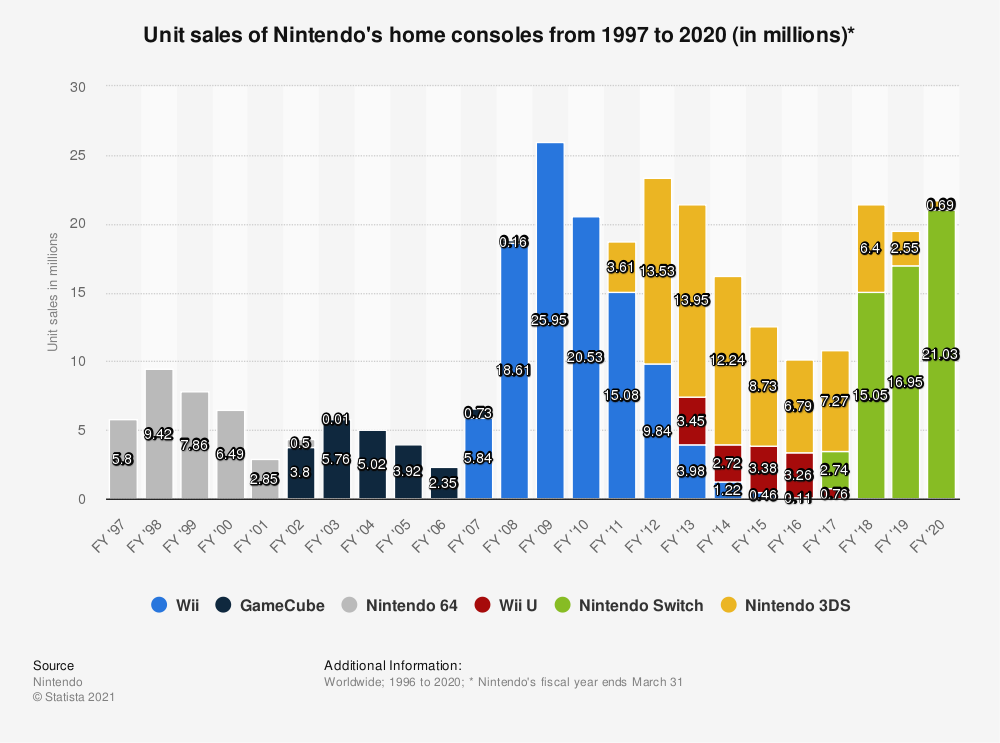
\includegraphics[scale=0.38]{kepek/nintendos-unit-sales-of-video-game-consoles-1997-2020.png}
			%	\caption{Nintendo otthoni konzolainak eladási statisztikája 1997-2020-ig}
			%	\label{fig:nintendos-unit-sales-of-video-game-consoles-1997-2020}
			%\end{figure}
		
			Másrészről, a Sony kifejlesztette 1994-ben az első CD-alapú konzolt, a PlayStation-t, mely erősségei közé sorolhatjuk a 3 dimenziós grafikát, valamint a CD-ROM technológia által adott hang- és képminőséget. A konzol képes volt nem csak a játékok futtatására, hanem emellett audio CD-k lejátszására is. A PlayStation-nel már szándékosan nem csak a gyerekeket, hanem a felnőttebb korosztályt is megcélozta a Sony, ebben az időszakban kezdett hétköznapivá válni idősebbek körében is ez a fajta szórakozási lehetőség. A PlayStation által ismerhettük meg a "Final Fantasy"-t, a "Tekken"-t, vagy épp a "Silent Hill"-t, melyek a mai napig ismert névnek számítanak.
			
			A PlayStation 2000-ben kiadta utódját, a 6. generációs konzolt, PlayStation 2 névvel (röviden: PS2), amely meglehetősen gyorsan népszerűvé vált. Több exkluzív név köthető hozzá, mely más platformon nem jelent meg. Egészen 2013-ig népszerű maradt, és folytatódott a gyártása, pedig akkorra már az utána következő PlayStation 3 is megjelent. A PS2 még napjainkban is a világ legnagyobb darabszámban értékesített konzolja.
			% TODO irodalom ->
			% https://hu.wikipedia.org/wiki/Vide%C3%B3j%C3%A1t%C3%A9k-konzol
			% https://hu.wikipedia.org/wiki/PlayStation_(konzol)
		\end{MySubSection}
		
		\begin{MySubSection}{Online játékok fejlődése}
			Korábban volt szó, az online játékokról, ennek elérésével többször próbálkoztak a fejlesztők, viszont hosszú ideig sikertelenül. Az első igazán népszerű online szerepjáték az 1997-es Massively Multiplayer Online Role-Playing Game (röviden: MMORPG) az Ultima Online volt, chat funkcióval, lehetővé téve a játékosok közötti interakciót és kommunikációt. Konzolok terén 2000-ben a Sega Dreamcast megjelentette első internetre-kész konzolját, egy igazán forradalmi rendszert, és az első internetes eszközt ami népszerűséget is szerzett. Azonban még ez is bukásra volt ítélve, tekintve, hogy még ekkor is kifejezetten költséges volt az internethozzáférés, így a Sega a felhasználók általi játék után hatalmas összegű számlákat kapott. A Sega kudarcának következtében a konkurens konzol-gyártók tanultak a negatívumokból, és a fejlesztéseiknek köszönhetően a 2000 körüli években az online funkcionalitás már nélkülözhetetlenné vált a játékiparban.
			% TODO irodalom ->
			% https://hu.wikipedia.org/wiki/MMORPG
		\end{MySubSection}
		
		\begin{MySubSection}{Technológia további fejlődése}
			A hardvergyártók egyre inkább felismerték a rengeteg potenciális üzleti lehetőséget, amik a multimédiás alkalmazásokban, videojátékokban rejlettek, rájöttek, hogy ezeken a területeken nagyobb teljesítményű hardverekre volt igény.
			A CPU (processzor) gyártók 2005 körülre már egyenesen a több magos processzorok felé haladtak. 
			GPU (videokártya) terén, az NVidia 1995 májusában jelentette be első grafikus kártyáját, az NV1-et, az ATI pedig szintén abban az évben, novemberben adta ki első 3D-s gyorsító kártyáját, a 3D Rage-et. Még azonban rengeteg problémával kellett megküzdeniük a gyártóknak. Az ATI 3D Rage végső változata, az ATI Rage 128 volt amely 1999-ben teljesedett ki. Ugyancsak 1999-ben látott napvilágot az NVidia GeForce 256 (avagy más néven NV10), amellyel az NVidia átvette a vezető szerepet a teljesítmény-versenyben.
			% TODO irodalom ->
			% https://www.techspot.com/article/650-history-of-the-gpu/
			% https://www.techspot.com/article/653-history-of-the-gpu-part-2/
			% https://hu.wikipedia.org/wiki/ATI_Technologies
			% https://hu.wikipedia.org/wiki/Nvidia
		
			Ezt megelőzően, amikor a számítógépek még nem tartalmaztak speciális, grafikai számítások gyorsítására használt feldolgozó egységet, még minden számítási feladatot a CPU végzett. Ezt a korai megjelenítési formát szoftveres raszterizációnak nevezzük. Ezzel a módszerrel tulajdonképpen a programozó teljes mértékben képes volt kezelni a megjelenítési folyamatokat, ami elég nagy rugalmasságot jelentett.
			Azonban a szoftveres raszterizáció hátránya, hogy nagyobb adathalmaz mozgatása és kezelése lassabban kivitelezhető a módszerrel, mint a grafikai processzorokkal.
			Ez azért fontos, mert a számítógépes grafikában lényeges célkitűzés volt a részletes, valósághű ábrázolás elérése, ami viszont nagy energiaforrásigényű, így a textúra szűréseket nem alkalmazó szoftveres megjelenítés, kimondottan egy 3D játék esetén lényeges eltérést mutatott már az első GPU-khoz képest is. \cite{mileff}
			% TODO irodalom -> 
			% https://users.iit.uni-miskolc.hu/~mileff/grafika/Grafika_programozasa_jegyzet_v0.66_Mileff_P.pdf
		
			A grafikai protesszorok megjelenése után, melyek tehát a valósidejű komplex kép kirajzolását gyorsítják, nagy lökést kapott a játékipar. Egyre inkább előtérbe kerültek a 3D-s játékok, mivel már volt lehetőség jobb minőségben elkészíteni őket, illetve a videokártya könnyen hozzáférhető volt és megfizethető, ezáltal gond nélkül elterjedt, a 3D-s játékok népszerűsége pedig azóta is töretlen.
			A hardvergyártás fejlődésének köszönhetően a videojátékok egyre filmszerűbbek és komplexebbek lettek, egyre inkább eladhatóvá váltak. Vegyük például a korábban említett Silent Hill-t, melynek atmoszféráját, a hangeffekteket, a grafikát kifejezetten eltalálta a PlayStation. Mindezek nélkül, más rendszerben, környezetben nem állta volna meg a helyét ennyire sikeresen ez a játék.
		
			A korábbi, hobbiból programozott játékok helyett jelentősen megnőtt az igény a modernebb, magasabb színvonalú játékfejlesztésre. 
			Így tehát a számítástechnika fejlődésével és az internet adottságainak jókora megnövekedésével, illetve elterjedésével egyre inkább jelentős részévé váltak a játékok a szórakoztatóiparnak, az előző generációt teljesen elsöpörve a fedélzetről.
		\end{MySubSection}
				
	\end{MySection}

	\begin{MySection}{Játékfejlesztés alapjai} 
		% TODO 	- játékfejlesztés alapjai ?
		% TODO 	- játékfejlesztés menete ?
		% pc
		
		\begin{MySubSection}{PC játékok}
			Fentebb már szó volt róla, hogy a számítógépes játékok az 1983-mas videojáték válság idején sokkal elterjedtebbé váltak, mint az egyéb platformokon lévők. 1984-re a számítógépes játékok vették át a vezetést a játék-piacon a konzolok helyett.
			% TODO irodalom ->
			% https://en.wikipedia.org/wiki/PC_game
			A csúcskategóriás PC-játékok szempontjából kifejezetten fontos, hogy a számítógépek általában sokkal több erőforrásssal rendelkeznek mint más játékrendszerek, platformok. A játékfejlesztők számára a jobb hardver lehetővé teszi a játékaik realisztikusabb és részletgazdagabb elkészítését a többi platformhoz viszonyítva. Itt gondolhatunk például részletesebb grafikai elemekre, melyet a nagyobb számítási kapacitás tesz lehetővé, vagy a gazdagabb felhasználói felületre, melyet a nagyobb felbontású megjelenítők, illetve a precízebben mozgatható egér használata tesz lehetővé. A felhasználói felületetes példánál maradva, egy konzolra nem érdemes olyan kezelőfelületet csinálni aminek sok menüpontja van, hiszen ott nincsen kurzor így a felhasználónak kényelmetlenül sokat kellene lépkednie mire egy kívánt ponthoz érne, míg a PC-n ezt akár egy egyszerű egérmozgatással is megoldhatja.
			Ha esetleg szeretnénk kipróbálni mennyire kényelmetlen is lenne egy ilyen kezelőfelület, próbáljuk meg használni a webböngészőnket, például egy google keresés találatai közti navigációra, egér használata nélkül, tabbal lépkedve a lehetséges elemek között.
			Azonban még ha ezekkel a lehetőséggekkel nem is élnek a fejlesztők, még mindig valószínűbb, hogy a számítógépen nagyobb képernyőfelbontáson, illetve jobb képfrissítés mellett tud futni ugyan az a játék.
			Ahogy már az előzőekből kikövetkeztethető, a számítógépeknél elsődlegesen az egér-billentyűzet kombinációt használják, de manapság már elterjedtek a joypadok vagy kontrollerek, illetve rendelkezésére állnak érintőképernyők és a mozgásvezérlők is. Ez a flexibilitás, melyet más platform nem (vagy csak részben) tudhat a magáénak szintén a PC előnyére válik. 
		\end{MySubSection}
	
		% mobil
		% TODO mobilhoz irodalom:
		% https://en.wikipedia.org/wiki/App_Store_(iOS/iPadOS)
		% https://www.marketsandmarkets.com/Market-Reports/mobile-applications-228.html
		% https://en.wikipedia.org/wiki/Smartphone
		
		\begin{MySubSection}{Mobil játékok}
		A mobilos játékok a 2000 körüli években kezdtek népszerűvé válni, azonban még csekély közönségük volt, egészen 2008-ig amikor az Apple elindította az App Store-t. Akkor még körülbelül 500 alkalmazást lehetett letölteni a telefonokra, mely mára már közel 2 millió applikációra bővült. Míg korábban szinte csak néhány vállalat uralta a játékpiacot, fokozatosan más cégek is bekerültek a képbe, például az Apple és Google, egyre növekvő eladásaikkal az alkalmazásboltjaikban. Az Apple például 2009-ben 2.5 billió letöltéssel uralta az alkalmazáspiacot. Az Apple sikere nagy mértékben elősegítette a globális alkalmazáspiac növekedését, fejlődését.
		A mobiltelefonok fejlődésének még egyik fontos mérföldköve volt az érintőképernyő. A 2000-res évek közepén már jelen volt a rezisztív érintőképernyő, amely reagált bármely nyomásra a felületen, tehát nem csak ujjal, hanem bármilyen eszközzel lehetett használni.
		% TODO irodalomjegyzékhez->
		% https://en.wikipedia.org/wiki/Resistive_touchscreen
		
		Az Apple által gyártott első okostelefon, az iPhone már kapacitív érintőképernyővel rendelkezett, ez a kijelző már nem minden eszközre reagál, ami hozzáér, hanem az emberi testre. Ennek a hátránya lehet, hogy hideg időben mondjuk ha kesztyűt hordunk, nem feltétlenül érzékeli az ujjunkat, viszont vannak "speciális" kesztyűk, amelyen keresztül érzékeli a képernyő az ujjhegyet, vagy pedig használhatunk speciális érintőtollakat is. 
		% TODO irodalomjegyzékhez->
		% https://en.wikipedia.org/wiki/Touchscreen
		Viszont előnye, hogy nem reagál mindenre ami hozzáér, például ha egy zsebben van, elkerülhetőek az esetleges véletlenszerű tárcsázások.
		Ezenfelül a képernyő méreteit is elkezdték nagyobbra gyártani, de mellette keskenyebbre. Az érintőképernyőn kívül kiemelendő még, hogy egyre erősebb hardvereket gyártottak. Jobb akkumlátorokkal rendelkező telefonokat bocsátottak piacra, egyre hosszabb üzemidővel.
		
		A mobiltelefonok fejlődése új lehetőségeket adott, és nem csak a játékfejlesztőknek. Manapság már rengeteg funkciót ellát a mobil, helyettesítheti például az órát, számológépet, fényképezőt, kamerát, GPS eszközöket, zseblámpát, hordozható játékeszközöket, és még tengernyi dolgot fel lehetne sorolni. Nem meglepő tehát, hogy az utóbbi 10 évben kifejezetten elterjedt az okostelefonok használata. 
		% TODO irodalomjegyzékhez->
		% https://www.itstimetologoff.com/2018/03/14/how-much-time-are-you-spending-on-your-smartphone/
		% https://flauntdigital.com/blog/evolution-mobile-phones/
		Egy 2017-es forrás alapján például megtudhatjuk, hogy akkoriban egy év alatt 700 és 800 óra közötti időtartamot telefonozott átlagosan egy ember, csak a 18-24 éveseket tekintve pedig ez a szám akár az 900-1000 órát is elérheti. Ezek a számok mind az android, mind az iPhone okostelefonokat tartalmazzák, az értékek pedig tovább is növekedhettek valamint növekedhetnek a jövőt tekintve is, mivel folyamatosan egyre több funkció és alkalmazás válik elérhetővé a felhasználók számára.
		
		% statisztikák
		A Statista 2019-ben publikált statisztikája szerint (lásd: \myref{fig:mobil:total_global_mobile_app_revenues_2014-2023} ábra) 2018-ban globálisan a mobil applikációk bevételének összege több mint 365 billió USA-dollár volt, illetve az ábrán látható az is, hogy a jövőre nézve milyen értékeket becsültek, egészen 2023-ig. Az alkalmazásokon belüli hirdetések, valamint a fizetős alkalmazások által nyert bevételt egyaránt tartalmazzák ezek a számok.
		% TODO irodalomjegyzékhez:
		% https://www.statista.com/statistics/269025/worldwide-mobile-app-revenue-forecast/
		\begin{figure}[h!]
			\centering
			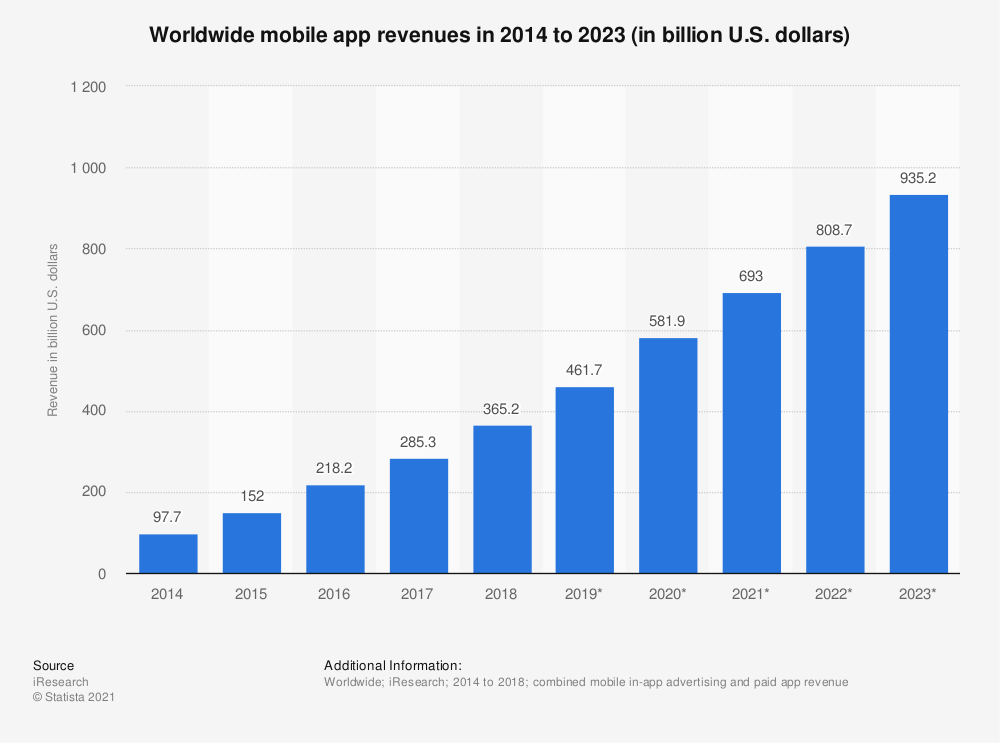
\includegraphics[scale=0.38]{kepek/mobil/total_global_mobile_app_revenues_2014-2023.png}
			\caption{A mobil alkalmazások bevétele 2014 és 2023 között világszerte}
			\label{fig:mobil:total_global_mobile_app_revenues_2014-2023}
		\end{figure}
		
		Egy 2021-ben publikált statisztikája alapján pedig megfigyelhető a Statistán, hogy 2016 és 2020 között hogyan változott a mobilos alkalmazások letöltésének száma, az egész világot beleértve (lásd: \myref{fig:mobil:annual_number_of_global_mobile_app_downloads_2016-2020} ábra).
		% TODO irodalomjegyzékhez->
		% https://www.statista.com/statistics/271644/worldwide-free-and-paid-mobile-app-store-downloads/
		\begin{figure}[h!]
			\centering
			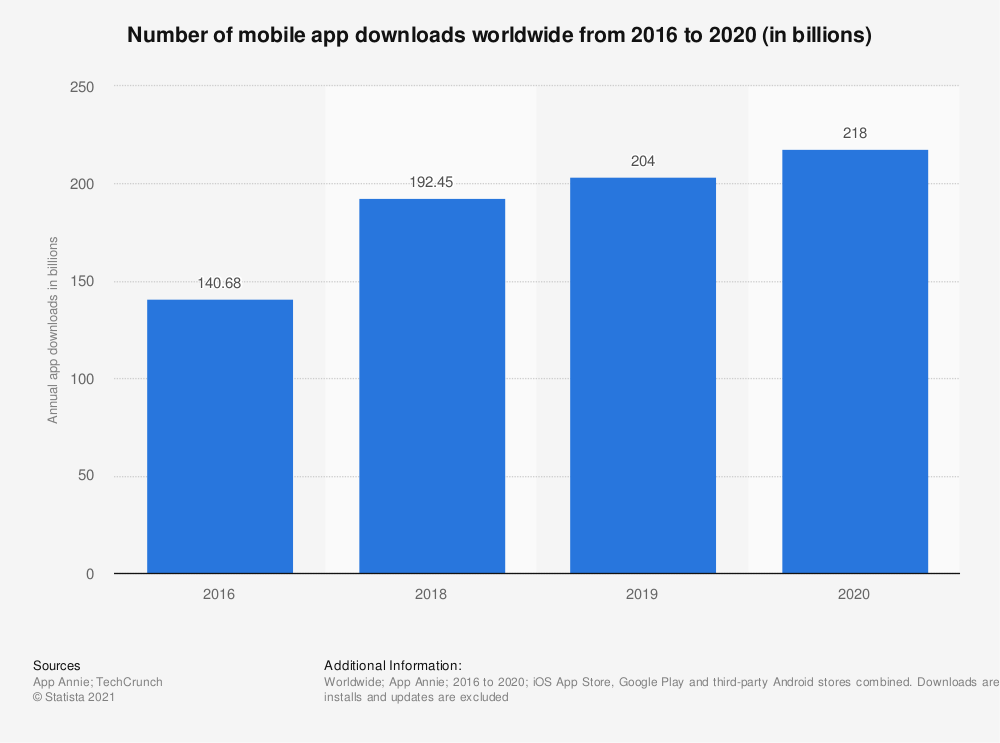
\includegraphics[scale=0.40]{kepek/mobil/annual_number_of_global_mobile_app_downloads_2016-2020.png}
			\caption{2016 és 2020 közötti mobilos alkalmazás letöltések száma világszerte}
			\label{fig:mobil:annual_number_of_global_mobile_app_downloads_2016-2020}
		\end{figure}
	
		Itt csak a legelső letöltésekre értendő az érték, az újratelepítéseket, valamint a frissítéseket már nem tartalmazzák ezek a számok. Ezenkívül megemlítendő még, hogy nem csak a két legnagyobb letöltésszámú alkalmazásbolt (azaz az iOS App Store és a Google Play), hanem az egyéb Android boltok is részt vesznek a statisztikában, mind a fizetős, mind pedig az ingyenesen letölthető alkalmazásaikkal. Közel 80 billiós emelkedést figyelhetünk meg az értékeken 2020-ra, a 2016-os 140,7 billió letöltésszámhoz képest.
		
		Ezenkívül megfigyelhetjük nem csak általánosságban a mobil applikációk, vagy a mobilos játékok bevételét, hanem összességében a játékokét is a különféle platformokon, illetve még néhány fontosabb mérföldkövet a mobilok világában (lásd: \myref{fig:mobil:Rise_of_Mobile_Gaming_Visualized} ábra).
		\begin{figure}[h!]
			\centering
			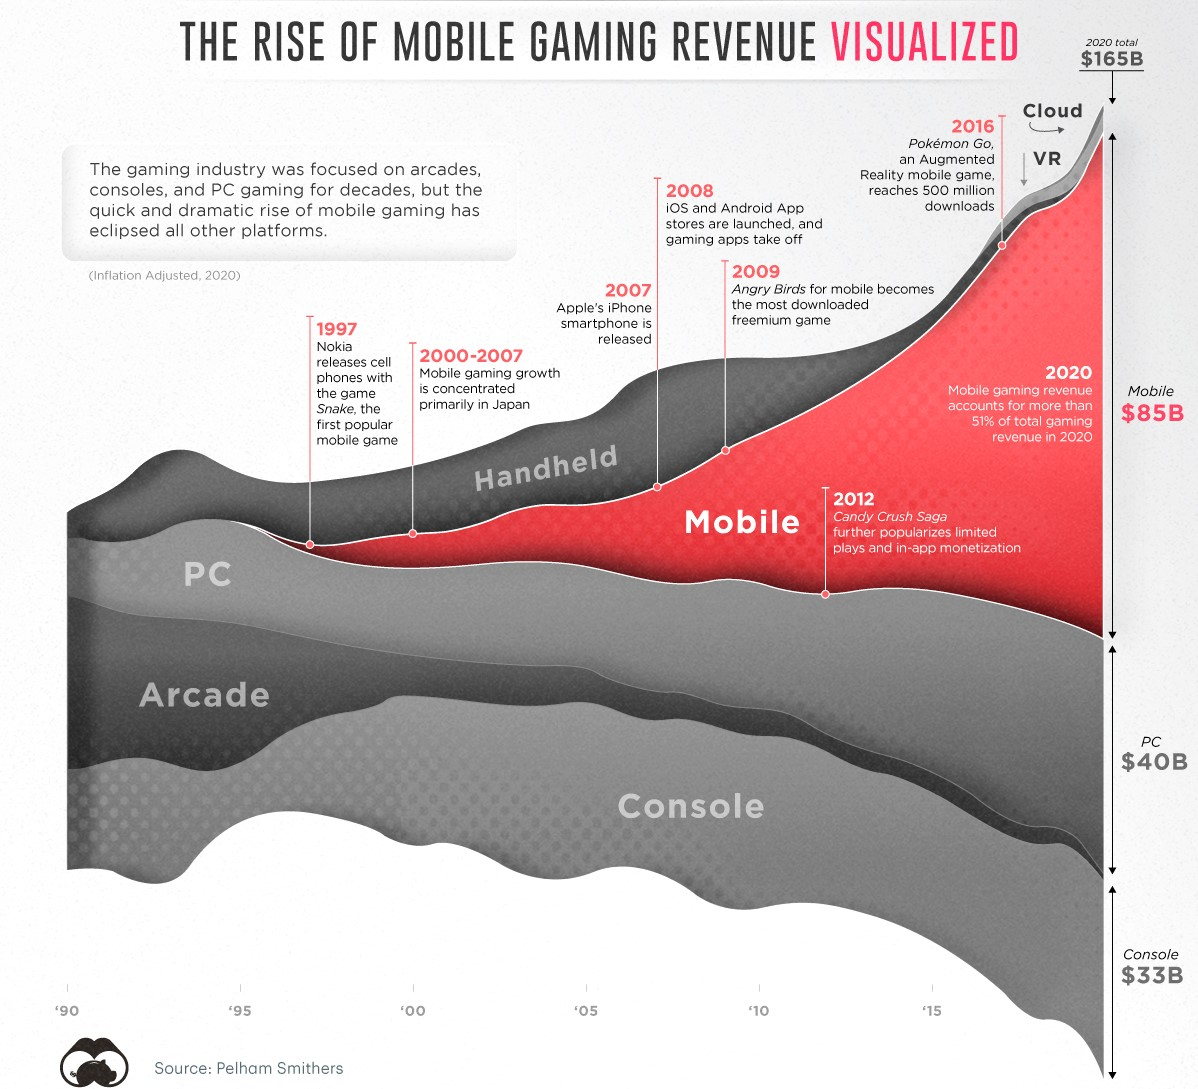
\includegraphics[scale=0.34]{kepek/mobil/Rise_of_Mobile_Gaming_Visualized.jpg}
			\caption{Mobil játékok elterjedése 1997-2020}
			\label{fig:mobil:Rise_of_Mobile_Gaming_Visualized}
		\end{figure}
		% TODO irodalomjegyzékhez->
		% https://www.visualcapitalist.com/how-big-is-the-global-mobile-gaming-industry/
		
		Az illusztráción jól látható a tendencia: a mobil platformok egyre nagyobb részét hódítják el az iparágnak. Ezért mindenképp érdemes lehet elgondolkodni, hogy egy leendő játékot milyen platformon készítünk el. Ha nem is elsődlegesen mobilra készül a játék, akkor is érdemes lehet valamilyen változatban (lebutítva, vagy más mechanikákkal kiegészítve) mobilra is kiadni azt.
		Jó példa lehetne erre a Fallout Shelter 2015-ből, amely a kezdetektől fogva mobilra is készült, vagy a League of Legends, ami eredetileg PC-re lett kiadva, azonban nemrég (2020 októberében) elkészült egy mobilos változata is, feltehetően pontosan azért, hogy a platform hatalmas játékosbázisát felhasználva még több emberhez juttassák el a játékot, és hogy ne csak a számítógép előtt ülve, de akár utazás közben is könnyedén játszhassanak a felhasználók, a gyártók pedig ezzel még több profitra tegyenek szert.

		% egyéb lehetőségek mobillal: képernyő megosztása tv-re
		A mai okostelefonokkal azonban rengeteg egyéb lehetőségünk is adódik, melyek közül párat meg is említenék, a játékokhoz kapcsolódóan. A különböző platformok, illetve a gyártók közötti határokon megfigyelhetjük, hogy már kevésbé különülnek el egymástól.
		Manapság már egyszerre konzolt és telefont is használhatnak a felhasználók egyes játékok, platformok irányításához. Például bizonyos mobilos játékokat ma már módunkban áll PlayStation kontrollerrel vezérelni. Másik hasonló lehetőség napjainkban, hogy maga az okostelefon is használható vezérlőként TV-hez és számítógéphez egyaránt, vagy akár billentyűzetet is alkalmazhatunk konzolok irányításához.
		
		Megfigyelhető, hogy egy adott játék sok esetben több különféle platformon is elérhető. A mobilos felhasználók körében igény mutakozhat arra, hogy egy konzol illetve PC játék elérhető legyen mobilon is, de fordított esetben már kevésbé merül fel ilyen igény. Például egy mobil játékot nem feltétlenül szeretne a felhasználó számítógépen játszani, hiszen a mobil könnyebben hozzáférhető, szinte mindig nálunk van, utazás közben is egyszerűen használhatjuk, játszhatunk rajta, míg a konzolokről és a PC-kről ez nem mondható el. Viszont ha mégis nagyobb képernyőn szeretnénk látni a mobilos játékot, ezt is könnyedén elérhetjük. Mostanság szinte minden háztartásban van TV készülék, és a mai technológiának köszönhetően a TV-nken is tudunk például Android játékokkal játszani, ezenkívül egyszerűen kivetíthető a telefon képernyője TV-re (vagy épp PC-re), így játszhatunk az eszközön telefonos játékokkal is.
		% TODO irodalomjegyzék->
		% https://gadget-info.com/66728-15-best-android-tv-games-you-should-play
		% https://www.origo.hu/techbazis/20150826-android-tv-sony-bravia-4k-google-operacios-rendszer-alkalmazasok-uj-orulet.html
		% https://www.cnet.com/how-to/unified-remote-turns-your-android-into-a-pc-controller/
		% TODO 	-sokan: mobil app-nak álcáznak weboldalakat (ma már számos- html5 js ts) de valójában html alapú, csak egy app-ba van becsomagolva <- ezekről pár oldal	(ionic, react native, etc) js-es alkalmazást weben/androidon ios-en akár windowson is futtathatóvá teszi PL discord
		\end{MySubSection}

		% ->végül nem ide lesz írva -webes(általánosan, később részletezve)		
		% TODO 	-hardveres gyorsítós böngészős játékok
		% TODO 	-elérhető technológiák / irányok
		% TODO 	-Jövő: a javascript mert az futtatható mindenhol (ha nem túl erőforrás igényes az alkalmazás)
	\end{MySection}

	\begin{MySection}{Játékfejlesztés keretrendszerek nélkül}
		% c++, low-level 
		Keretrendszerek nélküli fejlesztés esetén rendszerint inkább alacsonyabb szintű programozási nyelveken fejlesztenek, mint például a C++, mert általában eleve a sebesség miatt nem alkalmaznak keretrendszert, ezért feltehetően olyan programozási nyelvet használnak mellé, ami elősegíti azt, hogy gyorsan futó kódot tudjunk írni.
		
		Keretrendszer nélküli fejlesztéskor a megjelenítéshez használhatunk API-kat (Application Programming Interface rövidítése, ez gyakorlatilag megkönnyíti a fejlesztők munkáját azzal, hogy adott programok vagy programrendszerek szolgáltatásainak dokumentációjához, utasításkészletéhez nyújtanak hozzáférést), mint például az OpenGL (Open Graphics Library). Az OpenGL egy platformfüggetlen, alacsony szintű API, melyet 1992-ben fejlesztett ki egy amerikai cég, a Silicon Graphics. Segítségével szinte közvetlenül vezérelhetjük a grafikus kártyát, programozhatjuk a 3D-s grafikát, 3 dimenziós alakzatokat rajzolhatunk ki. 
		Manapság inkább tervezésben, gépészetben, valamint gyártásban használják, játékokban már kevésbé, főképp a viszonylag bonyolult használata miatt. Azonban fontosnak tartottam megemlíteni itt, mivel egy időben még ez volt az egyik legnépszerűbb megjelenítéshez használatos API játékok terén is, illetve a mai modernebb technológiák közül is rengetegnek az OpenGL szolgált alapjául.
		% TODO 	-a fentebb leírt opengl-es cucc jó így??
		% Megemlítendő az OpenGL, mert ez az egyik legrégebbi, tulajdonképpen azért fontos megemlíteni mert egy alap motor.
		%- open-source, - platformfüggetlen, bármilyen oprendszeren működik az opengl-es alkalmazás, leginkább a videokártya határozza meg h milyen funkciókat lehet vele használni. 
		% opengl bonyolult használat, kevésbé népszerű, már jobb és gyorsabb megoldások is vannak
		% nem feltétlenül szokták játékfejlesztéshez használni, mert bonyolultabb dolgokat nehéz benne összerakni, de egyszerűbb játékokhoz, vagy akár csak szemléltetéshez példákhoz ezt is lehet használni.
		% már van modernebb verziója is, aminek már jobb a teljesítménye, de még továbbra sem terjedt el eléggé ahhoz, hogy nagyobb projekthez érdemes legyen számításba venni.		-> még ha ugyan olyan jó is lenne mint a többi, mivel kevesen használják, ha problémába ütközöl feltehetően magadtól kell megoldanod, mert nem feltétlenül találsz rá megoldást az interneten
		
		% előny
		A keretrendszerek nélküli játékfejlesztésnek a sebességen kívül is számos előnye lehet a használatukkal szemben, főleg tapasztaltabb fejlesztők számára, többek között:
		\begin{itemize}
			\item Itt mindent saját magának készít el a fejlesztő, ezért ez a fejlesztési módszer kevésbé kötött, nagyobb rugalmasságot ad.
			\item Egy idő után, ha sokat fejlesztünk játékmotorok használata nélkül, kialakul egy általunk fejlesztett "keretrendszer". Ez persze nem biztos, hogy valóban egy komplett játékmotor, viszont azon amit tartalmaz könnyedén kiigazodhatunk, mert egyből tudjuk, mit hol kell keresnünk a kódban.
			\item Főleg az előző ok miatt, ha hibát ejtünk valahol, könnyebb kijavítani.
		\end{itemize}
	
		% hátrány
		Kezdő, tapasztalatlanabb játékfejlesztők számára azonban hátrány lehet, hogy ez a folyamat sokkal lassabb, időigényesebb lehet, mint egy már meglévő motor használatával elkészített alkalmazás.

		% TODO 	- példa ilyenre
	\end{MySection}

	\begin{MySection}{Játékfejlesztés keretrendszerekkel}
		% game-engine mit tartalmaz
		A keretrendszerek, azaz a grafikus motorok és a játékmotorok használata a 2000 körüli években vált kimondottan gyakorivá, nagy lökést kaptak a grafikus processzorok megjelenése után.
		
		A grafikus-, valamint a játékmotorokat céljainktól függően fontos megkülönböztetnünk egymástól, ez funkcionalitásuk szerint egyszerűen kivitelezhető:
		\begin{itemize}
			\item Grafikus motorok csak képi megjelenítésben segítik a programozót.
			\item Játékmotorok ennél bővebb, egy nagyobb eszközrendszert biztosítanak a fejlesztőknek.
		\end{itemize}
		% előny
		Mivel játékfejlesztéshez egy játékmotor használata a célszerűbb, mint a grafikus motoré, ezért a fejezetben főleg a játékmotorokról lesz szó bővebben.
		A játékmotorok használata tehát előnyös lehet az effektívebb, gyorsabb játékfejlesztéshez. Mivel a számítógépes grafika magas szinten van, szükség lehet a motor komplex funkcionalitására. A technológia fejlődése által egyre szebb látványvilágot tudnak visszaadni mind a grafikus-, mind a játékmotorok. Használatukkal viszont rengeteg erőforrás megspórolható azzal, hogy nem a fejlesztő feladata megvalósítani például a fizikai alrendszert, ütközésvizsgálatot, a megjelenítésért felelős rendszert, stb.
		Nem csak az egész játékmotort egyben, hanem önmagában csak egy-egy alrendszert is lehetőségünk van megvásárolni, mely abban az esetben lehet például kifizetődő, ha egy már kipróbált, megfelelő alrendszert beszerezni olcsóbb, mint egy saját, új alrendszer kifejlesztése. \cite{mileff}
		% TODO irodalom -> 
		% https://users.iit.uni-miskolc.hu/~mileff/grafika/Grafika_programozasa_jegyzet_v0.66_Mileff_P.pdf
		A mobilok megjelenésével új terület nyílt meg a keretrendszerek számára, több ismert játékmotort forgalmazó cég hordozható eszközökre elérhető változatot is adott ki.
		Keretrendszert használhatunk számítógépre, konzolra, valamint mobil eszközre való fejlesztésre egyaránt, a célplatformtól függően számos motor közül válogathatunk. Létezik külön 2D-s valamint 3D-s alkalmazás fejlesztéséhez megfelelő játékmotor, illetve van, amelyik mindkettőre alkalmas.
		
		% hátrány
		A fentebb említett főbb előnyei miatt, egy modern motor vásárlása nagy költséget jelenthet a fejlesztők számára, ami nem meglepő, mert nagyon sok munka van az elkészítésében.
		Az esetlegesen magas áron felül, hátránya lehet még, hogy a fejlesztésben kevesebb rugalmasság, szabadság van, illetve nehezebb kijavítani az esetleges hibákat fejlesztés közben.
		
		\begin{MySubSection}{Mai ismertebb keretrendszerek}
		% game-engine-k
		Napjainkban számos játékfejlesztésre (és egyéb alkalmazások fejlesztésére) alkalmas keretrendszer megtalálható a piacon, mint már szó volt róla, több platform terén is.
		\newline \newline
		Ezek közül példaként néhány közkedvelt:
		\begin{itemize}
			\item CryEngine
			\item Unity
			\item Unreal Engine
			\item Source
		\end{itemize}
		Természetesen ennél sokkal több játékmotor létezik, melyeket az interneten könnyedén megtalálhatunk, és néhányat akár ingyenesen is letölthetünk.
		Például a következő linken: \url{https://en.wikipedia.org/wiki/List\_of\_game\_engines} találhatunk a Wikipédián egy listát rengeteg keretrendszerről (a teljesség igénye nélkül), ahol a nevüket, az elsődleges programozási nyelvüket, a célplatformjukat, az adott játékmotor közreműködésével elkészült játékok listáját, valamint egyéb tényezőket is megtekinthetünk.
		
		A fentebb említett motorok közül kettőről alább láthatunk egy-egy rövid bemutatást, néhány főbb jellemzőt.
		\end{MySubSection}
	
		% unity
		\begin{MySubSection}{Unity}
			Vegyük példának az egyik népszerű, modern játékmotorra a Unity Technologies által fejlesztett Unity-t, melyet 2005-ben adtak ki először. A motor C\# nyelvet használ a programozáshoz.
			
			Az előnyei közé sorolhatjuk, hogy alapvetően ingyenes, számos hasznos funkcióval, részletes, jól használható dokumentációval rendelkezik, és kimondottan sok platformot támogat. Emellett egy Asset Store-ral is rendelkezik, amelyben jó néhány hasznos dolgot találhatunk, például textúrákat, modelleket, animációkat, stb.
			
			Megemlítendő még, hogy az ingyenes verzióján túl, elérhető a Unity Pro, egy fizetős változata is, mely több funkcióval rendelkezik.
			Hátránya lehet, hogy nem nyílt forráskódú.
			
			Összességében azonban egy rendkívül pozitív visszajelzésekkel rendelkező, igazán ígéretes motornak mondanám. Különösképp javasolt a használata, ha azt szeretnénk, hogy a készített játékunk sok, különféle platformon elérhető legyen.
			% TODO irodalom -> 
			% https://www.gamedesigning.org/engines/unity-vs-unreal/
			% https://unity.com/
			% https://en.wikipedia.org/wiki/Unity_(game_engine)

		\end{MySubSection}
		
		\begin{MySubSection}{Unreal Engine}
		% unreal engine
		Egy másik kitűnő játékmotor az Unreal Engine. A motort 1995-ben kezdte el írni az Epic Games (amerikai játék-, illetve szoftverfejlesztő és kiadó cég) alapítója, név szerint Tim Sweeney. Eredetileg azzal a céllal, hogy elősegítse egy játék fejlesztési folyamatát, amely Unreal névvel jelent meg, több év után, 1998-ban. Az Unreal nevű játék egy First-Person Shooter (röviden: FPS, ez a műfaj magyarul belső nézetű lövöldözős játékot jelent), kezdetben tehát a motor FPS játékok fejlesztéséhez íródott. Azóta viszont rengeteget fejlődött, és már számos népszerű játék készült el a segítségével, nem csak FPS, hanem egyéb kategóriákban is, például MMORPG (azaz a már korábban említett többszereplős online szerepjátékműfaj), vagy platformer játékok (ide sorolható minden olyan játék, melynek nagy részét képezi a platformokon való ugrálás).
		
		A motor egyik főbb jellegzetessége, hogy grafikai szempontból igazán fejlett. Nagyobb projektekhez is ajánlatos a használata, hiszen a motor alapvetően C++ nyelvet alkalmaz programozás terén, ezzel is elősegítve a teljesítményt, gyorsaságot.
		
		Maga a játékmotor ingyenesen letölthető és hasznáható játékok készítéséhez, azonban ha ki szeretnénk adni egy Unreal Engine-ben készült játékunkat, amennyiben az sikeres lesz, egy bizonyos mennyiségű bevétel után már 5\%-nyi szerzői jogdíjat kell fizetnünk.
		
		A keretrendszer fejlődésén jelenleg is dolgoznak, a következő verziójából, az Unreal Engine 5-ből már nyilvánosságra is hoztak egy kis ízelítőt, a teljes verziót pedig a 2021-es év végére tervezik kiadni.
		% TODO irodalom ->
		% https://en.wikipedia.org/wiki/Unreal_Engine
		% https://www.unrealengine.com/en-US/blog/a-first-look-at-unreal-engine-5
		% https://en.wikipedia.org/wiki/Epic_Games
		% https://hu.wikipedia.org/wiki/First-person_shooter
		% https://www.google.com/search?tbm=bks&q=isbn:9780429560576
		% példák
		A fejlődés szemléltetéseként mellékelek egy-egy fotót a motor régebbi verziójával készült, 2001-ben PlayStationre kiadott Harry Potter és a bölcsek köve játékról (lásd: \myref{fig:unrealEngine:harry-potter-and-the-sorcerer-s-stone-ps} ábra), valamint az Unreal Engine 5 által készített PlayStation 5-ön futó demóról, mely 2020-ban látott napvilágot (lásd: \myref{fig:unrealEngine:First-look-at-Unreal_Engine_5} ábra). A platform tehát mindkét esetben konzol volt, viszont a technológia fejlődése kifejezetten szembetűnő, a 2001-es, illetve a majdnem 20 évvel későbbi fénykép között.
		\begin{figure}[h!]
			\centering
			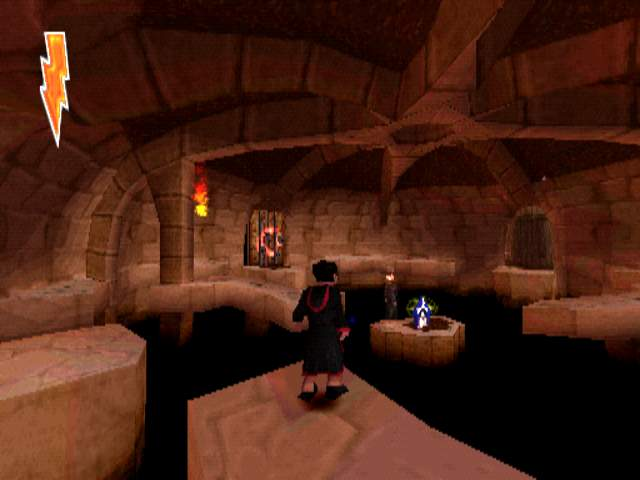
\includegraphics[scale=0.4]{kepek/unrealEngine/harry-potter-and-the-sorcerer-s-stone-ps.jpeg}
			\caption{Harry Potter és a bölcsek köve PlayStation játék (2001)}
			\label{fig:unrealEngine:harry-potter-and-the-sorcerer-s-stone-ps}
		\end{figure}
		\begin{figure}[h!]
			\centering
			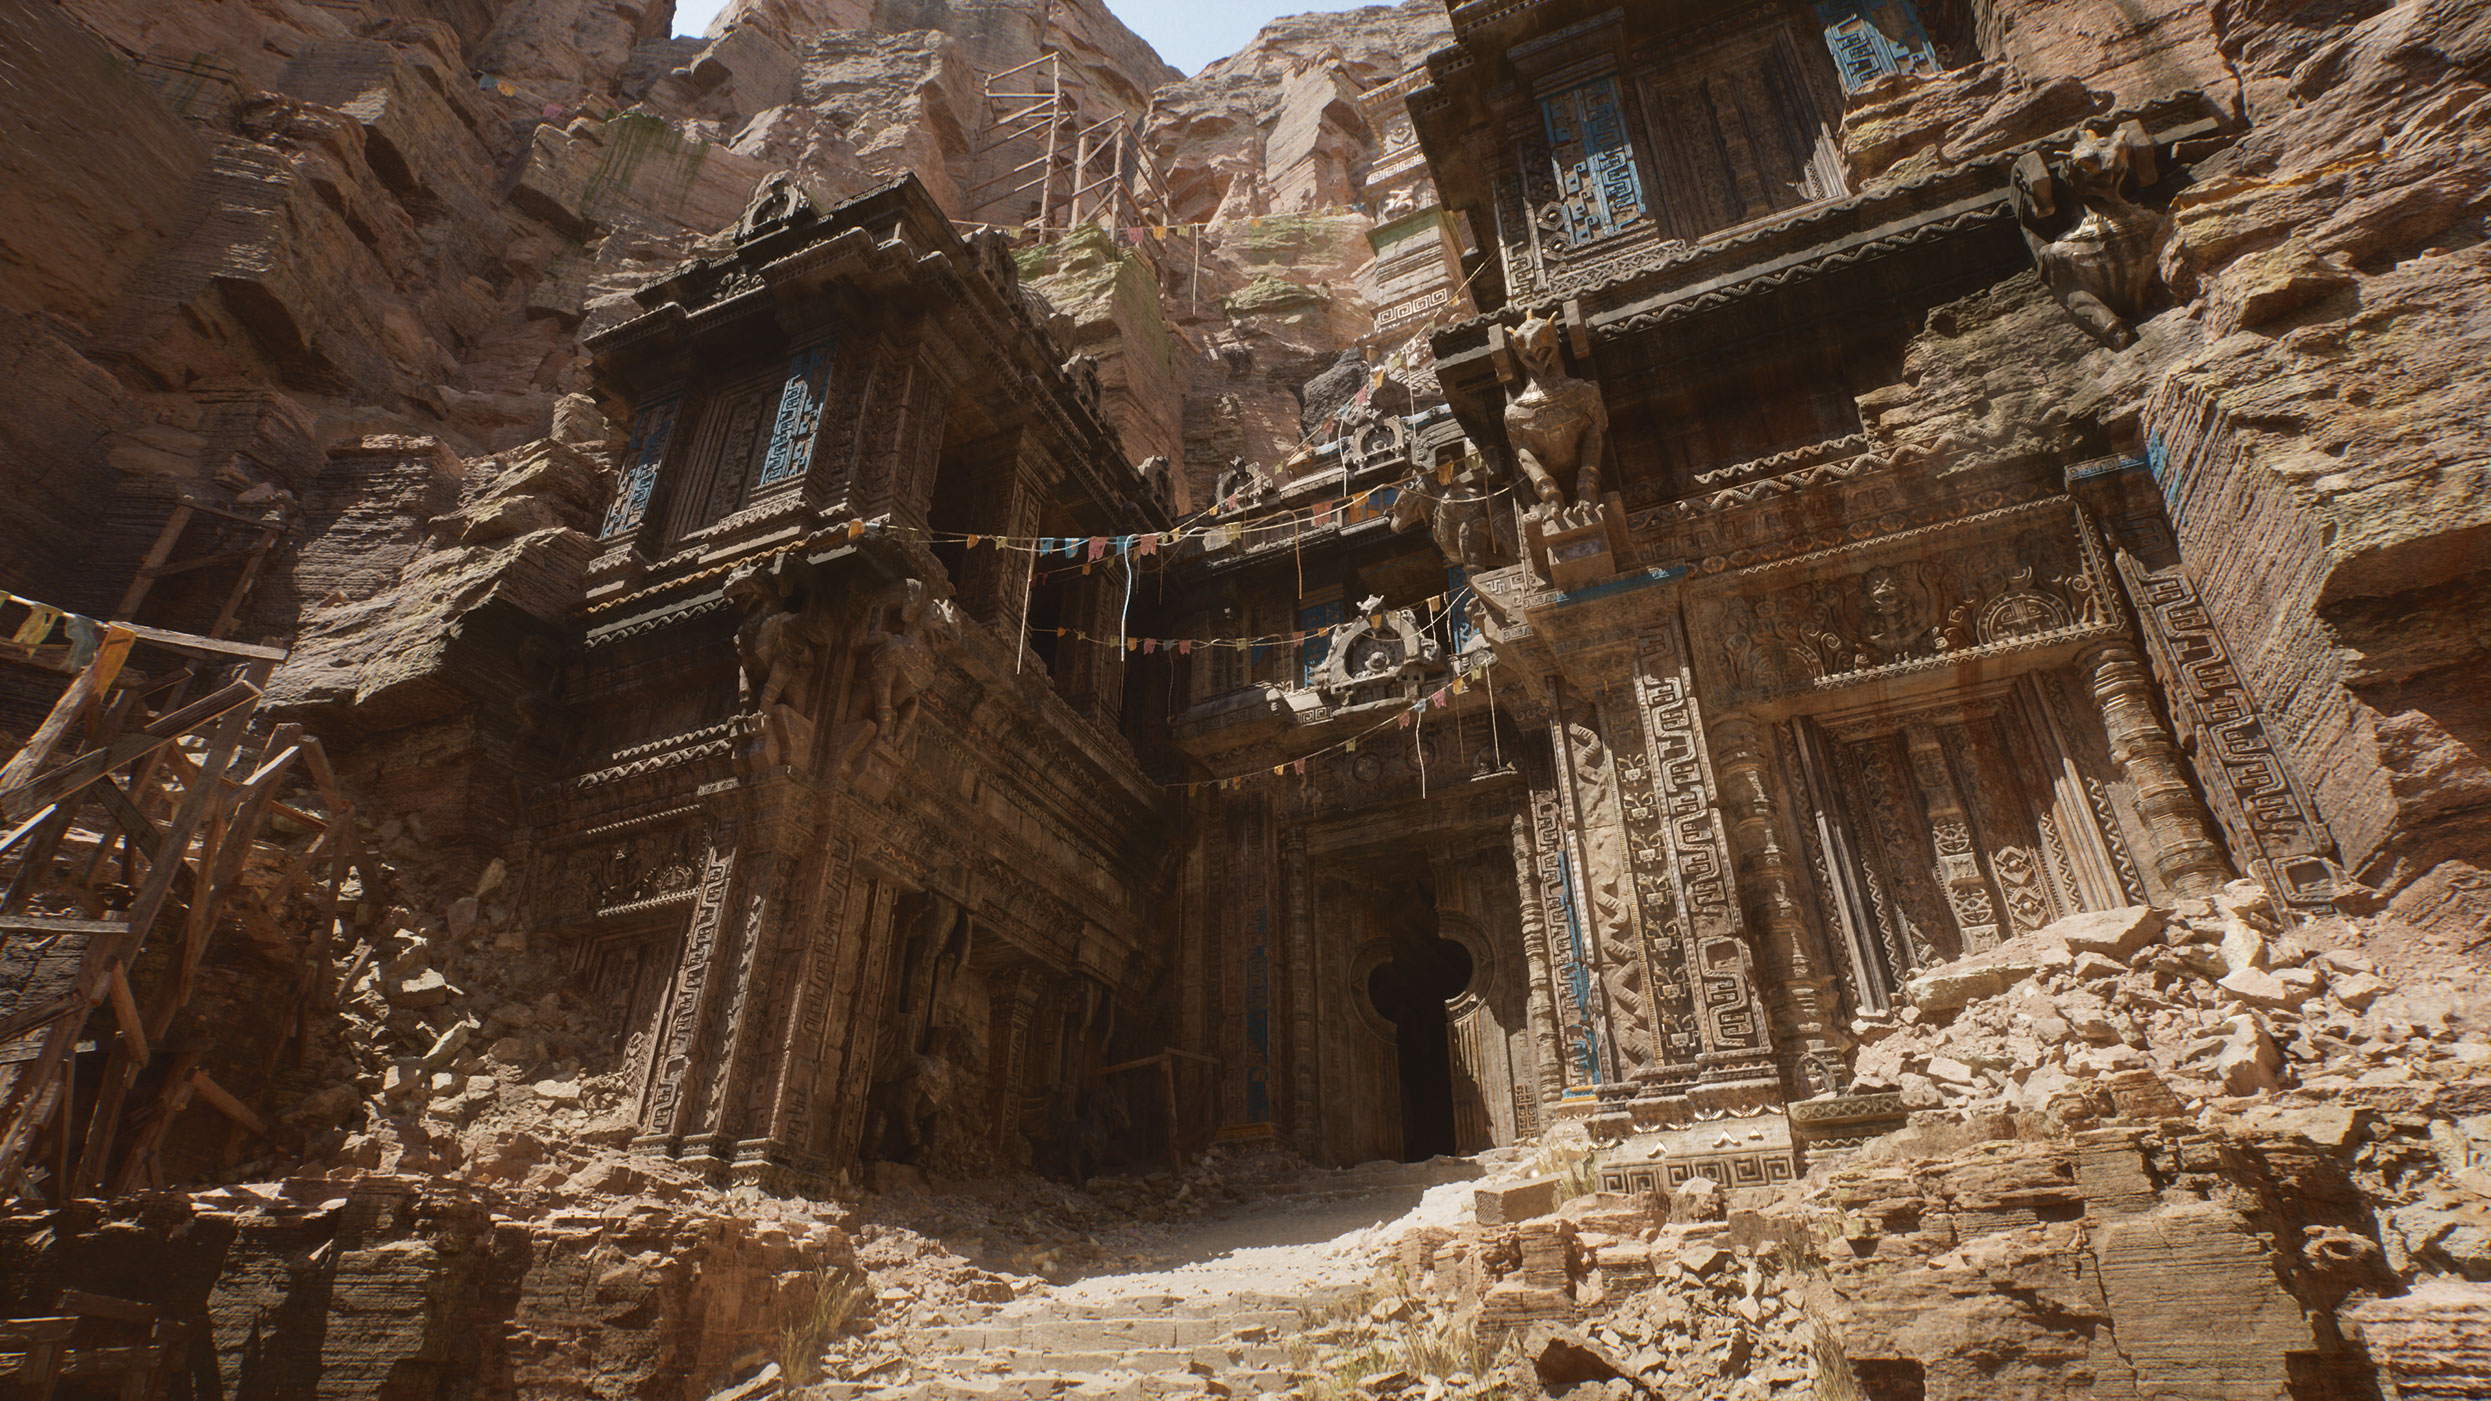
\includegraphics[scale=0.16]{kepek/unrealEngine/First-look-at-Unreal_Engine_5.jpg}
			\caption{Unreal Engine 5 demó (2020)}
			\label{fig:unrealEngine:First-look-at-Unreal_Engine_5}
		\end{figure}
	
		A képeket szemügyre véve tisztán látható a különbség, hogy az újabb változata a keretrendszernek mennyivel filmszerűbb, részlegtagazdabb látványvilágot képes nyújtani.
		% TODO forrás->
		% https://tcrf.net/Prerelease:Harry_Potter_and_the_Sorcerer%27s_Stone_(PlayStation)
		% https://www.unrealengine.com/en-US/blog/a-first-look-at-unreal-engine-5
		\end{MySubSection}
		
		% TODO 	- telepítésük
		% TODO 	- használatuk
		% TODO 	- tapasztalatok (kipróbálás ha lehet)
		% TODO 	(- összehasonlítás, konklúzió)
		% TODO - táblázatos formában összehasonlítás esetleg?
		
		% TODO 	- statisztikák, kezelhetőség, tanulhatóság, gyorsaság stb
		\end{MySection}
	
\end{MyChapter}
\begin{MyChapter}{Játékfejlesztés webes alapokon}	
	% TODO - leírni mi lesz a fejezetben
	% TODO - először szót kell ejteni néhány témáról: html5, stb: melyek a webes környezet miatt kapcsolódnak a játékfejlesztéshez is.

	\begin{MySection}{Webes fejlesztés}
		% TODO 	- kialakulása, néhánya általános dolog
		
		Az internet fejlődésével a böngészőkben játszható játékok nem csak helyet kaptak, de szinte a legnagyobb közönséghez jutottak el. A hozzáférésük sokkal könnyebb, mint a boltokban megvásárolt játékoknak, hiszen szimplán csak egy webcímre szükséges ellátogatni, majd magában a böngészőben zajlik a játékmenet. Napjainkban pedig az eszközeink nagy részén már rendelkezésre áll egy böngésző. Ezen felül a szociális hálózatok elterjedése szintén felgyorsította a böngészős játékok egyre több emberhez való eljutását.
		
		% TODO irodalomjegyz.->
 		% https://en.wikipedia.org/wiki/Browser_game
		% https://www.awwwards.com/current-state-and-the-future-of-html5-games.html
		% https://docs.microsoft.com/en-us/archive/msdn-magazine/2015/march/game-development-a-web-game-in-an-hour
		
		Azonban a böngészők erőforrásai kifejezetten korlátozottak voltak, komplexebb alkalmazásokhoz már nem biztosítottak elég funkciót. Ezért a fejlesztők különböző cégek által készített plug-in-eket, programokat használtak, mint például a Microsoft Silverlight, vagy az Adobe Flash. Ezek a kiegészítések már komolyabb grafikus tartalom megjelenítésére voltak képesek, viszont az összes használónak szükséges telepítenie a megfelelő plug-in-t. 
		
		% TODO a webes fejl. fejezet végére:
		Kijelenthetjük tehát, hogy a mai modern kornak és a webes szabványoknak köszönhetően, ma már böngészőbe épülő plug-in-ok nélkül is képesek vagyunk modern hardveresen gyorsított számítógépes grafika, illetve a felhasználói elvárásokat kielégítő szintű játékok készítésére.
	\end{MySection}

	\begin{MySection}{HTML5}
		% TODO	- mi ez, miért jobb mint ami eddig volt
		Korábban már szó volt róla, hogy a HTML5 fő célja a fentebb említett funkcióknak az egységesítése volt, anélkül, hogy a felhasználóknak különböző plug-in-eket kellene használniuk ahhoz, hogy megfelelően működjenek az egyes elemek a böngészőben.
		A funkciók szabványosítása folyamatosan zajlik, így bár már most is megfelelő felületet nyújt a webes játékok, alkalmazások számára, a jövőben még ennél is népszerűbbé válhat.
		A HTML5 és JavaScript alapú technológiák előkelő helyet foglalnak el platformfüggetlenség terén, viszont fontos megjegyezni, hogy ezzel a technológiával egy összetettebb, nagyobb adattartalommal rendelkező játékot (ma még legalábbis) nem feltétlenül érdemes elkészíteni, mert könnyedén megizzaszthatja nem csak az átalgos felhasználók számítógépeit, hanem akár a modernebb gépeket is.
	\end{MySection}

	\begin{MySection}{JavaScript}
		% TODO 	- mi ez, miért jó
		% TODO 	- kialakulása
		A JavaScript (röviden: JS) egy kis erőforrás-igényű, objektum-orientált programozási nyelv, mely lehetőséget nyújt a fejlesztők számára a weboldalaikba való komplexebb dolgok implementálására. Amennyiben olyan weblapról beszélünk, amely nem statikus tartalommal rendelkezik, hanem interaktív tartalom is megtalálható rajta, akár 2D-s vagy 3D-s animáció, stb., abban az esetben valószínűsíthető, hogy JavaScriptet is tartalmaz az oldal. Ezenkívül, bár webes tartalmaknál használják a leggyakrabban, számos webböngészőn kívüli környezetben is alkalmazható. A nyelvet eredetileg 1996-ban fejlesztették ki, azóta sokat változott, a szintaxisa közelebb került a Java programozási nyelvhez. Az ECMA (Európai informatikai és kommunikációs rendszerek szabványosítási szövetsége) először 1997 és 1999 között szabványosította ECMAScript néven.
		% TODO irodalom ->
		% https://developer.mozilla.org/en-US/docs/Learn/JavaScript
		% https://hu.wikipedia.org/wiki/JavaScript
		% https://developer.mozilla.org/hu/docs/Web/JavaScript
		% https://hu.wikipedia.org/wiki/Ecma_International
		% https://wiki.prog.hu/wiki/JavaScript
		% https://data-flair.training/blogs/advantages-disadvantages-javascript/
		A JavaScript főbb jellemzői:
		\begin{itemize}
			\item A futási környezete többnyire egy webböngésző.
			\item Lehetőséget ad az interaktivitásra. (Ezalatt a felhasználó által megvalósított események kezelhetőségére gondoljunk.)
			\item A legtöbb böngészővel kompatibilis, emiatt népszerű is.
			\item A kiszolgáló tehermentesítését is elősegíti: Űrlapküldés esetén küldéskor megvizsgálhatja, hogy az összes űrlapmező ki van-e töltve. Amennyiben nincs, a kliens oldalon fel tudja hívni a felhasználó figyelmét erre.
			\item Sokoldalú, mivel alkalmas front-end és backend fejlesztésre, valamint weboldalak vagy webapplikációk tesztelésére egyaránt.
		\end{itemize}
		Összességében elmondhatjuk, hogy a JavaScript szinte mindenhol futtatható, rengeteg helyen alkalmazzák, és ezalatt a front-end valamint a back-end mellett a mobil, az asztali, illetve a hibrid alkalmazásokat is érthetjük. A nyelv kifejezetten népszerű, folyamatosan fejlődik, a webfejlesztés egyik vezető programnyelve és feltehetőleg még hosszú ideig így is marad.
		% TODO irodalomjegyzék ->
		% https://www.creative-tim.com/blog/web-development/javascript-future-learn-javascript/
		% TODO megnézni h van e vmi hasznos ebben https://www.freecodecamp.org/news/future-of-javascript
	\end{MySection}

	\begin{MySection}{TypeScript}
		% TODO 	- mi ez, miért jó
		% TODO 	- kialakulása
		A TypeScript szintén egy objektum-orientált nyelv, tulajdonképpen a JavaScript típusokkal, osztályokkal, és egyéb hasznos funkciókkal kibővített változata. Tehát minden, amit JavaScript-ben megtehetünk, az TypeScript-ben is lehetséges, továbbá egy működő JavaScript kódot átvihetünk TypeScript kódba, az ott is le fog futni, a futási időben való viselkedés pedig nem fog változni, még akkor sem, ha a TypeScript úgy érzékeli, hogy a kód típushibákat tartalmaz. Fordítás során a TypeScript fájlok JavaScripté konvertálódnak át. A nyelvet a Microsoft készítette. Érdemes észrevennünk, hogy a TypeScript-ben található típusok, osztályok, privát illetve publikus láthatóságok, stb. ellenőrzése csak fordítási időben történik meg, futásidőben nem garantált.
		A TypeScript megjelenése előtt a JavaScript programozók gyakran követtek el típushibákat, még akár szimpla elgépelések miatt is. Ezen hibák kiküszöbölésével azonban a TypeScript hatékonyabbá teheti a JavaScript fejlesztést, nagyobb projektek esetében is.
		% TODO irodalom->
		% https://www.typescriptlang.org/
		
		A nyelv főbb jellemzői tehát a következők:
		\begin{itemize}
			\item Objektum-orientált programozási nyelv.
			\item Teljesen nyílt forráskódú.
			\item A fordító a TypeScript forráskódból JavaScript kódot generál.
			\item Operációsrendszer független valamint böngészőfüggetlen.
			\item Egy már meglévő JS kódot fel tudunk használni TypeScriptben, tehát felülről kompatibilis a JavaScript nyelvvel.
		\end{itemize}
		% TODO ESLint TSLint (PMD, Chechstyle Java esetén)
	\end{MySection}

	\begin{MySection}{Általános célú javascript keretrendszerek}
		% TODO 	- nem játékfejlesztéshez
		Korábban már volt szó a keretrendszerekről, melyeket játékfejlesztésre használhatunk, azonban természetesen léteznek ezeken túl is keretrendszerek. Néhány általános célú JavaScript keretrendszerről lesz szó a továbbiakban.
		Ha úgy döntünk, hogy használni szeretnénk például egy JS keretrendszert, rengeteg széles körben elterjedt, népszerű opció áll a rendelkezésünkre, és mindnek megvan a saját előnye, valamint hátránya, attól függően, hogy mi a fő célunk vele: például front-end, backend fejlesztés, vagy tesztelés. Emiatt nehéz lehet eldönteni, hogy vajon melyik is lenne tökéletes választás számunkra. A döntésben esetlegesen segítségünkre lehetnek a különféle keretrendszerek népszerűségével kapcsolatos statisztikák. Ehhez rendelkezésünkre állhatnak különböző források az interneten (például a következő weboldal: https://bestofjs.org/)
		Az említett weblapon nyomon követhetjük a felhasználók általi használat alapján a napi, heti, havi vagy akár az éves legnépszerűbb keretrendszereket.
		% TODO irodalom --->
		% https://www.lambdatest.com/blog/best-javascript-framework-2020/
		
		% TODO 	- angular, vue.js, react, egyéb
		Konkrét JavaScript keretrendszerek pedig például a Vue, React vagy az Angular. Ezek egyébként ebben a sorrendben 2017-ben az akkori év első három leghasználtabb JS keretrendszerei voltak a weboldal alapján, melyről fentebb szó volt.
		% TODO befejezni a vue-t
		A Vue egy nyílt forráskódú JavaScript keretrendszer, amely 2014-ben látott napvilágot, és azóta is az egyik legkedveltebb keretrendszer. A nyílt forráskódúság azért fontos szempont, mert ezek a keretrendszerek az elterjedt operációs rendszereken szinte biztosan elérhetőek.
		% TODO irodalom --->
		% https://skillcrush.com/blog/what-is-a-javascript-framework/
	\end{MySection}

	\begin{MySection}{Webes játékfejlesztés}
		% TODO itt a címet esetleg módosítani?
		% TODO 	- keretrendszerrel vagy nélküle
		% TODO 	- szükséges egyéb dolgok pl.: grafikai pakkok (al-al-fejezetek), hangok, texturák, objektumok
		
		Webes játékkészítéskor szükségünk lehet bizonyos plusz elemekre a játékunk elkészítéséhez, gondolhatunk itt textúrákra, felhasználói felülethez (GUI) szükséges elemekre, animációkra, audióra, stb. Amennyiben nem saját magunk szeretnénk elkészíteni ezeket a plusz dolgokat, az interneten rengeteg megfelelő grafikai pakk, asset (magyarul: forrás) található meg, rendelkezésünkre állnak mind fizetősek, mind ingyenesek. Ezek tehát lehetnek textúrák, hangok, animációk, sprite-ok, stb., két- és három dimenziós alkalmazásokhoz egyaránt. 
		
		A dimenziók száma meghatározó szerepet játszik abban, hogy milyen vizualizációs formát választunk a játékunk megjelenítéséhez. Mint később szó lesz róla, a szakdolgozat részeként egy 2D-s játékot készítek el, emiatt a három dimenziós grafikai megjelenítésekre most nem igazán fogok kitérni a fejezetben.
		
		Két dimenziós grafika esetén kimondottan elterjedt a Tile-Map alapú megjelenítési technika. Egyébként ehhez a módszerhez is számos asset lehet a segítségünkre az internetről. Az eljárás lényege, hogy kijelzőt virtuálisan azonos méretű úgynevezett Tile-okra bontjuk, és mivel ezeket a mezőket újra és újra felhasználjuk a felhasználó számára megjelenítendő háttérhez, ezért a memóriában helyet spórolhatunk meg azzal, hogy csak egyszer töltjük be az egyes tile-okat. A vizualizációs forma előnyei között tudható még, hogy akár nagyobb távolságra is valós időben lehetséges az útkeresés és az útvonal elaborálása, valamint (amennyiben az adott alkalmazáshoz elegendő a kisebb szintű vizuális komplexitás) viszonylag könnyedén kivitelezhető vele az ütközésvizsgálat.
		% TODO irodalom ->
		% https://users.iit.uni-miskolc.hu/~mileff/grafika/Grafika_programozasa_jegyzet_v0.66_Mileff_P.pdf
		A már elkészített és szétdarabolt tile-ok összességét Tileset-nek nevezzük. A Tileset-et leggyakrabban egy külön képben szokás tárolni. (Például így: \myref{fig:tileMap:tileSet} ábra)
		% TODO irodalom ->
		% http://higherorderfun.com/blog/2012/05/20/the-guide-to-implementing-2d-platformers/
		\begin{figure}[h!]
			\centering
			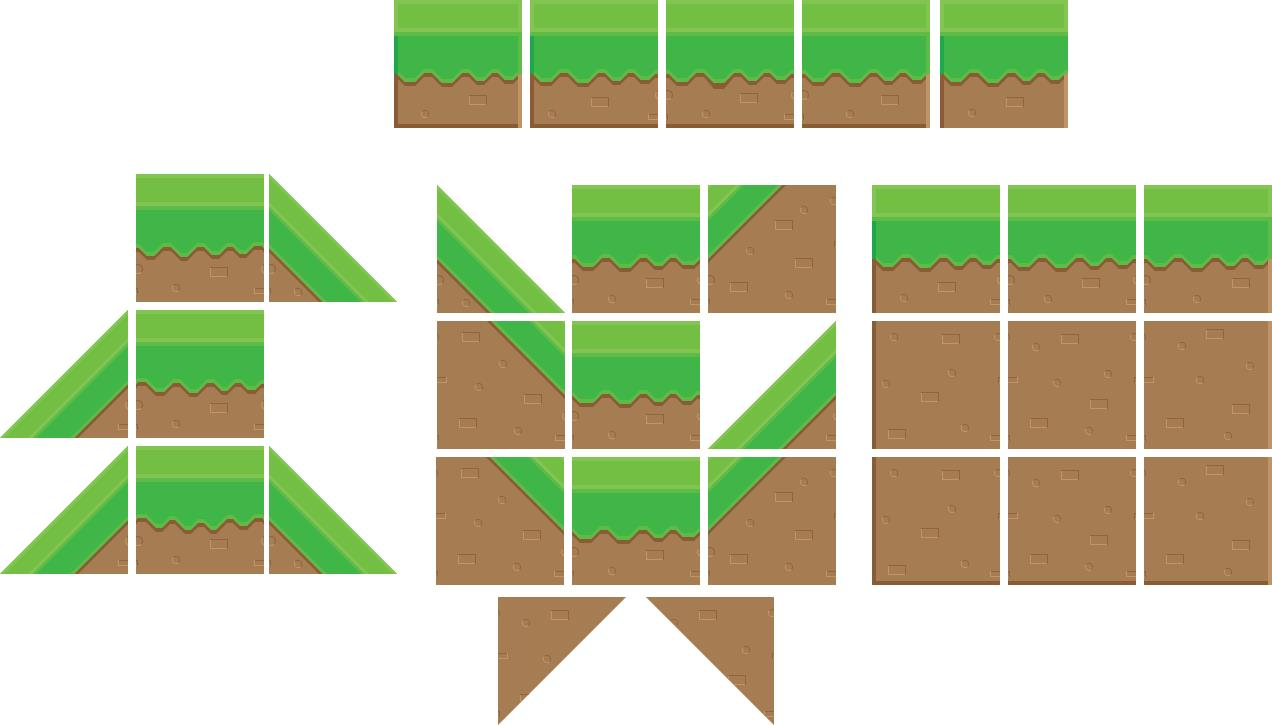
\includegraphics[scale=0.25]{kepek/tileMap/TileSet.png}
			\caption{Platform játékhoz alkalmas tileset}
			\label{fig:tileMap:tileSet}
		\end{figure}
	
		A Tile-Map alapú megjelenítésre a legalkalmasabb játéktípusok között vannak a felülnézetes, a puzzle, vagy például a platformer játékok. (A fentebbi tileset és egyéb elemek használatával példa a megjelenítési technikára: \myref{fig:tileMap:tileMapPreview} ábra)
		\begin{figure}[h!]
			\centering
			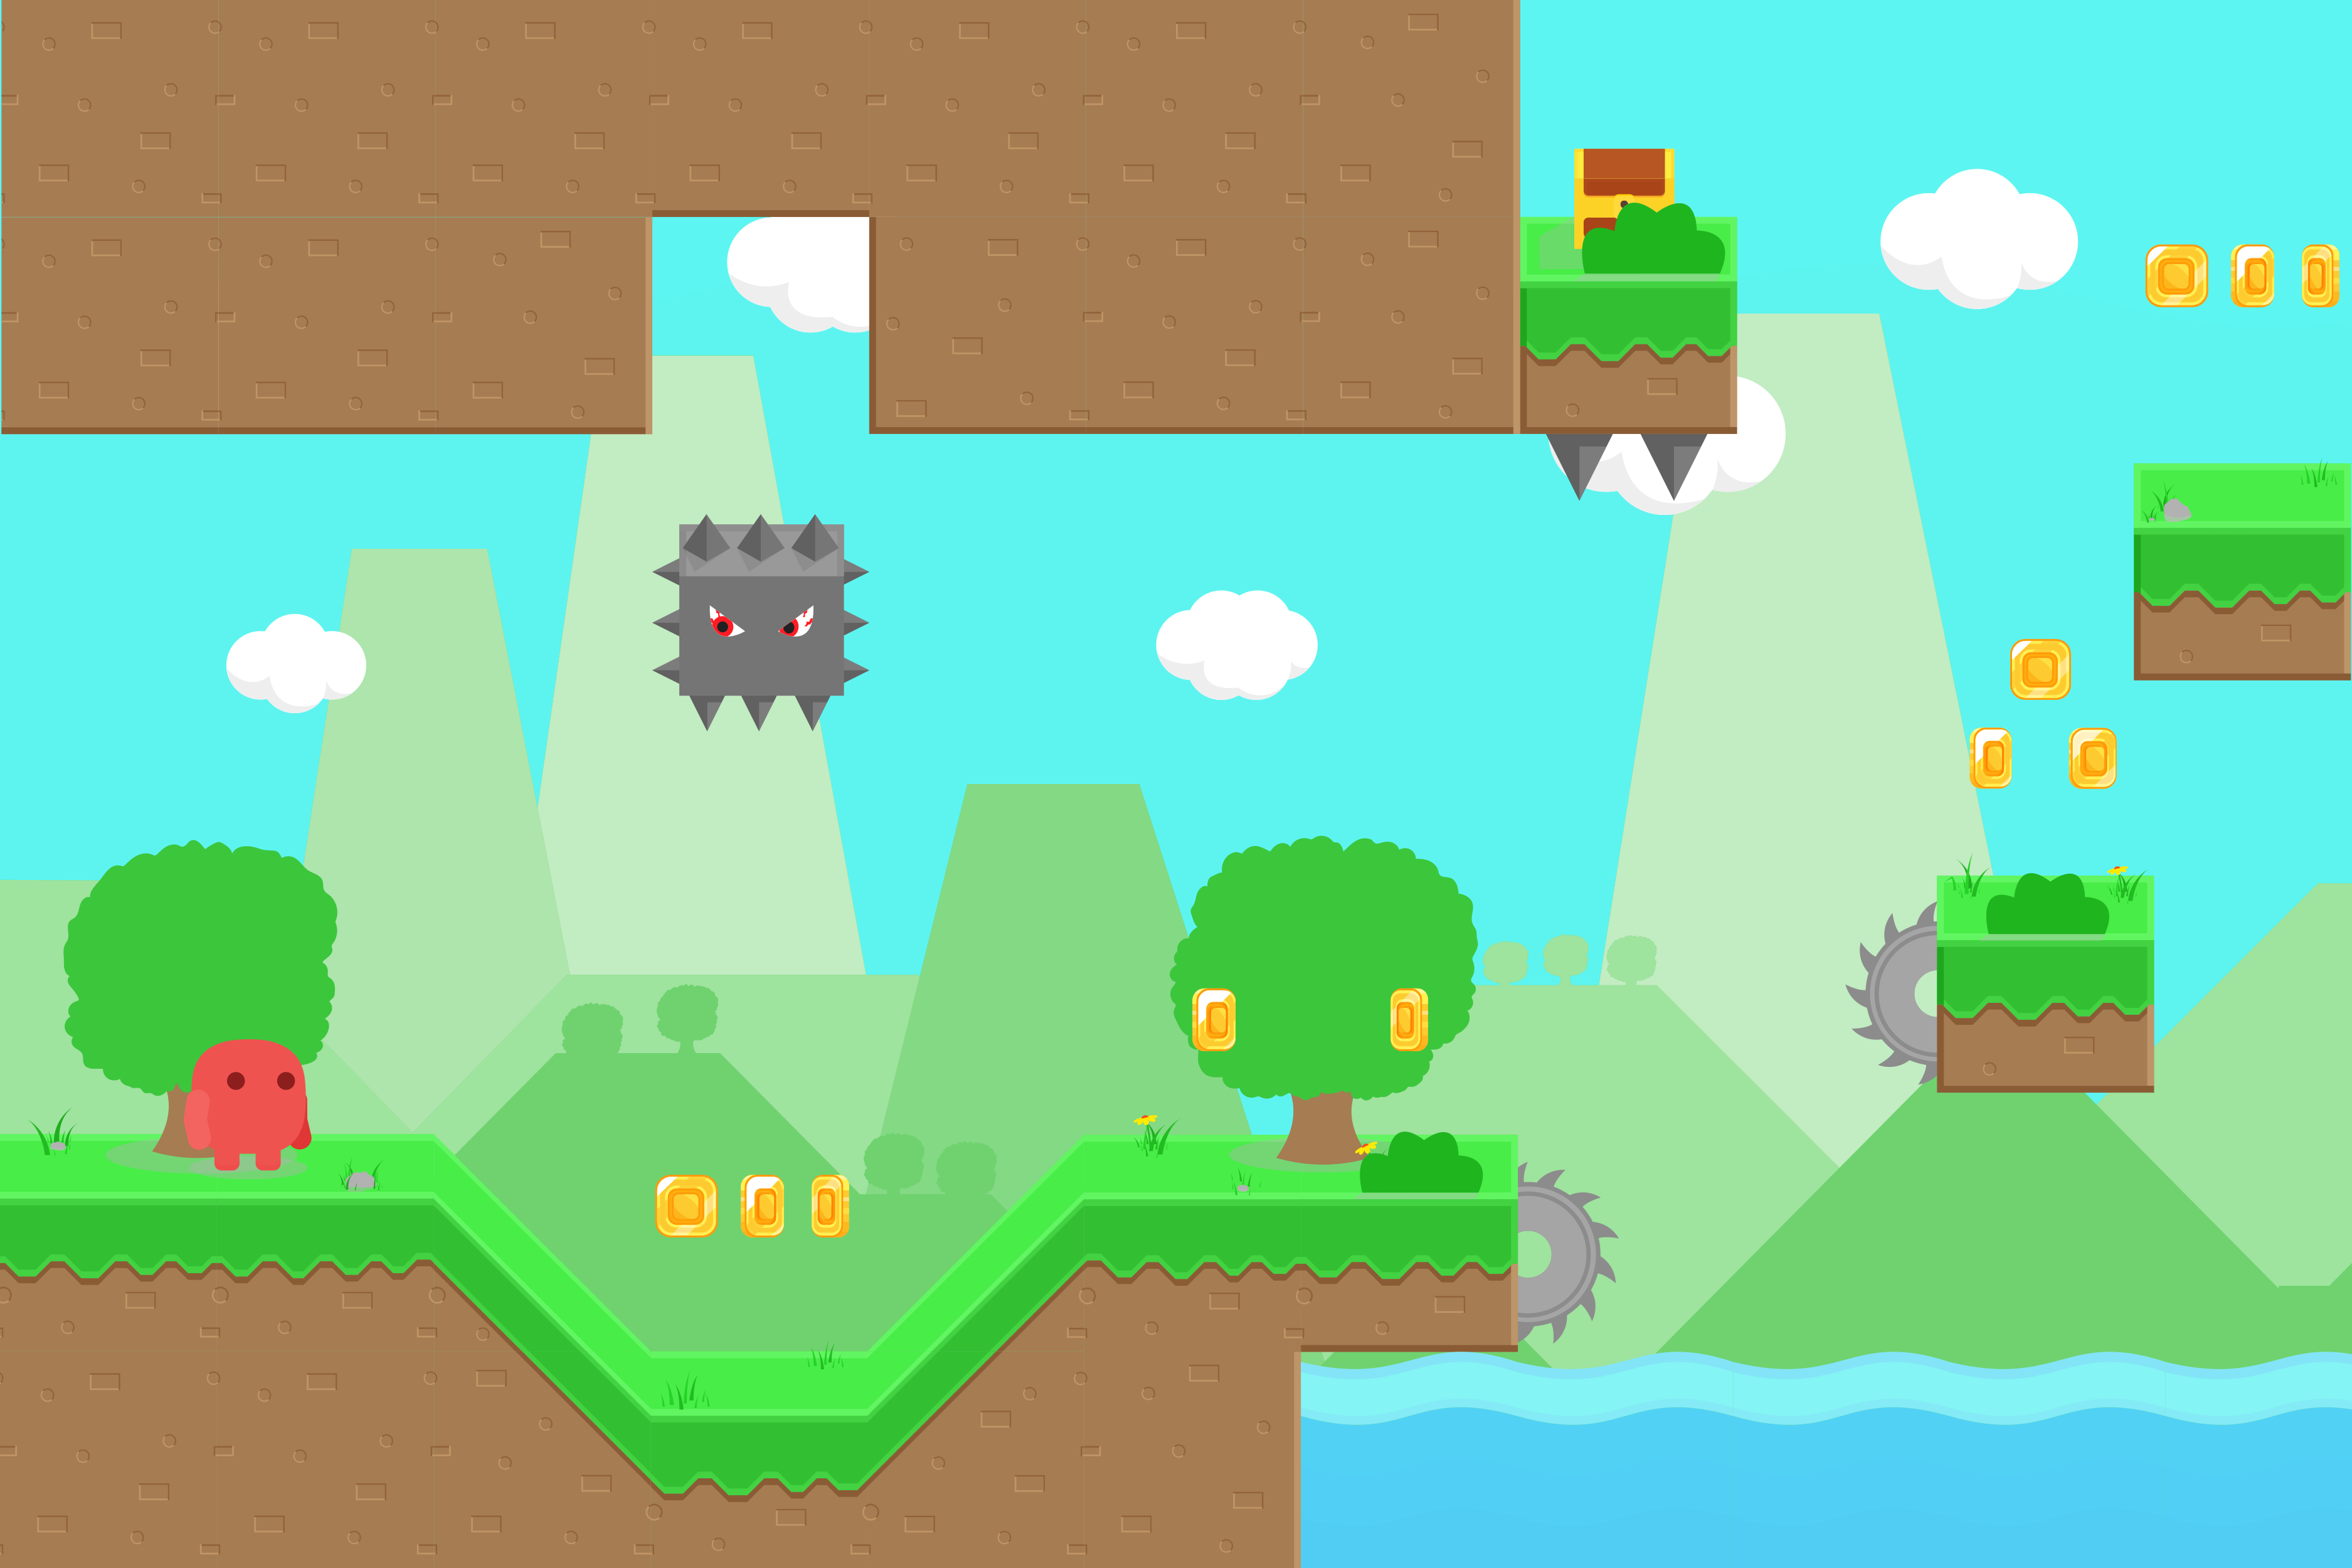
\includegraphics[scale=0.35]{kepek/tileMap/TileMapPreview.png}
			\caption{Példa tilesettel létrehozott platform játékra}
			\label{fig:tileMap:tileMapPreview}
		\end{figure}
		% TODO irodalom ->
		% https://bayat.itch.io/platform-game-assets
		% TODO 	- nem kell túl sokat ide írni, csak úgy általánosságban erről a dologról, mi kellhet hozzá
	\end{MySection}

	\begin{MySection}{Webes játékfejlesztés keretrendszerek nélkül}
		% TODO 	- "pure js"-ben
		% TODO 	- webgl
	\end{MySection}

	\begin{MySection}{Webes játékfejlesztés keretrendszerekkel}
		% TODO 	- keretrendszerek miért jók
		% TODO 	(- összehasonlítás menete(?))
		% TODO 	- felsorolni (tovább bontani al-al-fejezetekre ha megoldható)
		% TODO 	- megemlíteni melyik miért jó, miben más, használatuk, esetleg kipróbálás, személyes tapasztalatok
		% TODO 	- összehasonlítás eredménye / összegzése az előzőnek
		% TODO 	- dönteni melyiket használom -> Phaser 3
	\end{MySection}
	
\end{MyChapter}
\begin{MyChapter}{Saját játék fejlesztése}
	% mi lesz a fejezeteben
	A most következő fejezetben az általam fejlesztett alkalmazásról, avagy játékról lesz részletekbe menően szó. Mint már korábban említettem, egy program, alkalmazás vagy játék fejlesztésekor rengeteg opciónk van, mind a programozási nyelvet, mind pedig a felhasználandó technológiákat tekintve. Az én választásom végül arra esett, hogy egy keretrendszer segítségével készítek el egy játékot. A választott játékmotorral a \myref{Phaser} fejezetben találkoztunk már. Mivel még kifejezetten új számomra ez a terület, így jobbnak láttam, ha elsőként ezzel a módszerrel próbálkozom egy játék fejlesztésével, rengeteg ismeretet, tapasztalatot gyűjtve, azonban még nem saját motor készítésével együttesen.
	Tehát ebben a fejezetben elsőként ismertetem a céljaimat, azt, hogy mit is szeretnék majd elérni a játékkal, illetve hogy milyen elképzeléseim vannak a végeredményre vonatkozóan. Majd pedig be fogom mutatni, hogy hogyan indultam neki az elkészítésnek, valamint a felhasznált technológiákat, a tervezési, illetve a megvalósítási folyamatokat, stb. egyszóval részletezem az egész fejlesztési eljárást.
	
	\begin{MySection}{Célok meghatározása}
		% vázolni mit szeretnél elérni a programmal/játékkal, miről fog szólni, tehát az elképzelés (vízió dokumentum :) )
		Mint ahogy fentebb is szó volt róla, amellett döntöttem, hogy egy játékmotor használatával készítek el egy játékot. A választásom a Phaser 3 keretrendszerre esett, ahogy ez már az előző fejezetből kiderült.
		A szakdolgozatomban egy HTML5 alapú játék megtervezése és fejlesztése a célom, konkrétabban egy tower defense (magyarul: toronyvédő, röviden: TD) műfajú játék elkészítése. A TD játékok lényege, hogy a játékos tornyok, vagy egyéb objektumok építésével megakadályozza, hogy az ellenfelek, vagy szörnyek egy előre meghatározott ponton túljussanak. Egy ilyen műfajú játék egy felhasználó számára egyszerűen megtanulható, azonban igényel némi stratégiát, gondolkodást, ahogy egyre nehezedik. 
		% TODO irodalom ->
		% https://www.loopinsight.com/2010/03/30/understanding-tower-defense-games/
		% https://en.wikipedia.org/wiki/Tower_defense
		
		Azért választottam ezt a műfajt, mert egyrészt magam is szeretem az ilyesfajta stílusú játékokat, így amikor a tervezésén gondolkodtam, például azon, hogy milyen elemek legyenek benne, vagy hogyan haladjon a játékmenet, akkor rengeteg ötlet merült fel bennem, többek között emiatt is, hogy korábban már játszottam hasonló témájú játékokkal, és a korábbi tower defensekkel kapcsolatos tapasztalataim alapján pedig sokkal könnyebb volt eldönteni, hogy melyek azok a tulajdonságok, amiket egy efféle játékban fontosnak tartok. Ugyanakkor még kifejezetten segítségemre voltak ezek a játékélmények abban, hogy jobban meg tudjam határozni, hogy összességében milyen végeredményt szeretnék látni a saját játékomban, mind grafikai, mind pedig játékmenet szempontjából. Másrészt, mint már említettem, még nem igazán volt tapasztalatom játékok készítése terén, ezért egy egyszerűbb játékon keresztül szerettem volna megismerni a játékfejlesztést.
		
		Mindezek mellett a TD egy olyan játékműfaj, amely meglehetősen illeszkedik ahhoz az elképzelésemhez, hogy egy felülnézetes, két dimenziós játékot szeretnék készíteni. Vizualizációs forma terén pedig a Tile-Map alapú megjelenítési technikára esett a választásom, amely mint korábban már írtam is, kimondottan népszerű 2D-s grafika esetén. Az oka annak, hogy a két dimenziós grafikát preferálom szintén amiatt van, amit említettem nemrégiben, hogy egy visszafogottabb, egyszerűbb program készítésén keresztül szeretnék tapasztalatokat gyűjteni a játékfejlesztésről, ehhez pedig kevésbé lett volna alkalmas a 3D-s grafika.
		
		A játék alapkoncepciója az lenne, hogy az elején a főmenüből elindítunk egy pályát. Ezután betölt a pálya, ahol van egy meghatározott útvonal, amely egyik oldalán beérkeznek ellenfelek, a másik végén pedig ha túl sokan túljutnak, tehát nem sikerül őket megállítanunk, elpusztítanunk, akkor veszítünk. Az útvonalon kívül a pálya tartalmazna még egyéb objektumokat, tájelemeket, hogy ne legyen egyhangú a játék kinézete. Az ellenségek kiiktatásához tornyokat lehetne letenni amelyek támadják a szörnyeket. Az alapja ez lenne a játéknak, picit részletesebben a célok meghatározásáról pedig a továbbiakban fogok beszélni.
		
		Az elérendő célok közé sorolnám azt, hogy nem csak egy toronyfajtát szeretnék elérhetővé tenni, hanem többfélét, kinézetben és sebzési módban egyaránt különbözőeket. Ez utóbbit úgy kell érteni, hogy a tornyok, amiket elhelyezhetünk, amelyek támadni fogják az ellenfeleket, ne csak például egy golyót lőjenek ki, hanem szeretnék lézert, esetleg rakétavetőt, vagy más egyéb lövedékfajtát is. Fontos lehet még, hogy némelyik torony akár több szörnyet is tudjon egyszerre sebezni, például adott területre irányuló támadással, legfőképpen a játék későbbi szakaszában, amikor már különösen sok az ellenség. Mindenképp szeretnék effekteket is tenni a játékba, mondjuk olyat, ami lassítja az ellenfelet, ez segíthet főleg játék későbbi időszakában, hogy több ellenség legyen egy helyen, ezáltal még több szörnyet képesek lennénk támadni egyszerre, területi sebzéssel. Ezen effekteket esetleg vizuálisan is megkülönböztethetővé lehetne tenni, például lassítás esetén a szörny ami elszenvedi az effektet fagyos lenne, ha tűzzel kapcsolatos sebzést kap akkor pedig például lángolna egy darabig.
		Úgy gondolom, hogy az is hasznos lenne, hogy ha egyszer leteszünk egy tornyot, akkor nem feltétlenül kellene ott maradnia örökre, hanem akár lerombolhatnánk, ezzel valamennyi pénzt visszakapva, majd újat építhetnénk a helyére, ami erősebb, jobban illik oda az érkező ellenfelekhez. 
		
		Az szörnyek tömegben jönnének, bizonyos darabszám először, majd fokozatosan egyre több érkezne egy hullámmal. Minden új csoportnyi ellenség között egy kis időt szeretnék hagyni a legyőzésükre, és minden legyőzött csapat után nem csak több, de erősebb ellenfelek lennének a következő hordában. A felhasználó számára szeretném elérhetővé tenni azt, hogy éppen hanyadik hullám érkezik, valamint azt is, hogy hány szörnyből áll majd a következő csoportnyi ellenfél.
		Azon kívül, hogy meg tudjuk ölni az ellenséget a tornyok segítségével, lehetne mondjuk valamilyen objektumot az útjukba helyezni, ami megállítaná őket egy darabig, ez a lassítás effektű lövedéken túl szintén elősegíthetne egy területi sebzésű fegyvert.
		
		Mint ahogy az előző mondatból kiderülhet, szeretnék még valamiféle pénzrendszert, erőforrást vinni a játékba, amelyből megvásárolhatóak a tornyok a védekezéshez. A pénzt minden megölt szörnyeteg után kapja majd a játékos, és ide kerülne vissza az a pénz is amit visszakapnánk ha mondjuk lerombolunk egy tornyot. Bizonyos összegért esetleg el lehetne pusztítani egyes tájelemeket is, hogy ha nagyon rossz helyen vannak, a helyükre tudjunk tornyot tenni a védelem érdekében.
		
		A felhasználó számára láthatóvá szeretném tenni, hogy aktuálisan mennyi élete van, ezt növelni nem lehetne, viszont ezáltal egyértelmű lenne a játékosnak, hogy ha nem sikerült kiiktatnia egy-egy ellenfelet, ami így sikeresen végigment az egész útvonalon, illetve ebből az is világossá válik, hogy esetlegesen hány darab ellenség átengedése után veszítene.
		
		Emellett szeretnék még egy pontrendszert készíteni, minden megölt ellenfél után járna adott mennyiségű pont, csakúgy, mint a pénzgyűjtés esetében. A játékos természetesen ezt is látná, hogy az adott pályán a játék közben aktuálisan mennyi pontja van éppen, ezenkívül a játék végén is, még mielőtt a főmenübe visszatérne. Ezért ha esetleg valakiben túlteng a versenyszellem, akkor később javítani is tudna az eredményein.
		
		Az előző mondataimból már kiderülhet, hogy szeretném, hogy egy pályát akár többször is meg lehessen próbálni, viszont mindenképpen szükséges több pálya is, különféle útvonalakkal, mert különben hamar unalmassá, megszokássá válna főleg a játék eleje, ahogy mindig ugyanoda tehetnénk le csak a tornyokat, és folyton azonos útvonalon haladnának a szörnyek. Ezt elkerülendő tehát fontosnak tartom, hogy több pálya is legyen, például véletlenszerűen, vagy pedig a játékos által valamilyen bemenettel generálva. Ezáltal változatosabb útvonalak lehetnének, illetve a tájelemek sem mindig ugyanott helyezkednének el. A felhasználó számára feltétlenül módosíthatónak kellene lennie a generálásnak, vagy pedig a legutóbb alkotott pályát elérhetővé tenni, hogy ha ugyanazon az pályán szeretne játszani, például a magasabb pontszám elérése miatt, az megoldható legyen.
		
		% meddig szeretnék eljutni a játék készítésével
		Elsődlegesen azt szeretném elérni, hogy az alap funkcionalitás meglegyen, majd amikor az kész lesz, csak azután szeretném a fentebbi tulajdonságokból a lehető legtöbbet megvalósítani, kibővíteni a játékot. Gondolok itt arra, hogy például a vizuális effektek nem élveznek annyira prioritást. Ami még a célom, hogy a továbbiakban is lehetőség legyen bővítésre, illetve hogy az esetleges továbbfejlesztési lehetőségeket viszonylag könnyen intergálni tudjuk a programba a későbbiekben.
	\end{MySection}
		
	\begin{MySection}{Felhasznált eszközök, technológiák}
		% bármi (IDE, nyelv, OS, build-tool, git)
		A játék elkészítéséhez az alábbi technológiákat választottam, használtam:
		
		\begin{itemize}
			\item Phaser 3 - HTML5 alapú játékmotor (lásd: \myref{Phaser}).
			
			\item Windows 10 - Alapvetően a mindennapokban is Windows operációs rendszert használok elsősorban, emiatt azzal kapcsolatosan több tapasztalattal is rendelkezem, úgyhogy szinte természetes volt, hogy a játék fejlesztésekor is ezt az operációs rendszert szeretném használni.
			
			\item JavaScript - Alapjában véve a JavaScript mellett döntöttem, hiszen a programozási nyelv meghatározásánál lényeges volt szem előtt tartani, hogy a fejlesztéshez választott játékmotor mely nyelveket támogatja.
			
			\item TypeScript - A JavaScript alapvetően nem tartalmaz típusokat, pedig az valójában rendkívül megkönnyíti a fejlesztő dolgát, ennélfogva úgy határoztam, hogy a TypeScriptet is használom, ahol csak lehetőség van rá. Azonban mint írtam, a játékmotor nem teljesen kompatibilis a TypeScripttel, ebből kifolyólag nem lehet pusztán TS-t használni.
			
			\item Git - A program készítéséhez, főleg a nagysága miatt kétségkívül érdemes volt valamilyen verziókövető szoftvert alkalmazni. Azért a Git-et választottam erre a célra, mert a kisebb és nagyobb projektekhez egyaránt megfelelő, gyors, hatékony, kifejezetten jó a támogatottsága, és végül, de nem utolsósorban ingyenes. Mindezek mellett könnyen használható, a tanulmányaim során pedig egyébként is kellett már alkalmaznom korábban, így nem volt teljesen ismeretlen számomra a használata.
			
			\item Visual Studio Code - A Microsoft által fejlesztett, nyílt forráskódú kódszerkesztőt, a Visual Studio Code-ot (rövidítve VSCode, vagy VS Code) választottam integrált fejlesztői környezetként. A választásom okai közé tartozik, hogy a VSCode ingyenes, kis erőforrásigényű, de jól személyre szabható, és minden szükséges funkciót tudunk benne használni különféle plugin-ek segítségével.
			
			\item Node Package Manager - Röviden NPM, ez egy JavaScript csomagkezelő, melynek segítségével telepíthetjük, valamint kezelhetjük a csomagjainkat az alkalmazásunkhoz. % TODO Ez így jó, vagy átírni?
			
			\item Webpack bundler - Ez egy olyan program, mely egyrészt lefordítja a TypeScript kódot JavaScriptre, másrészt az így kapott forrásfájlokat egy fájlba csomagolja, tömöríti, optimalizálja, és az egyéb szükséges statikus fájlokkal, mint a HTML vagy képek, összelinkeli. Tehát röviden a kész alkalmazást rakja össze a forrásfájlokból.
			
			\item Jest - A manuális tesztelésen kívül még ezt a keretrendszert használtam teszteléshez.
			
			\item PlantUML - A PlantUML használatával sokkal hatékonyabban tudunk a program egyes részeiről UML diagramokat készíteni, így rengeteg időt lehet spórolni vele. Online elérhető az alábbi linken: \url{https://plantuml.com/}
			
			\item Photophea - Egy ingyenes, webalapú grafikus szerkesztő, mely az Adobe Photoshop-hoz hasonló. Alkalmas képek szerkesztésére, illusztrációk készítésére, különböző képformátumok közötti konvertálására, satöbbi.
			Számomra a képek, assetek módosítása, vágása miatt volt rá szükség.
			A következő linken érhetjük el: \url{https://www.photopea.com/} % TODO Ez így jó, vagy átírni?
			
			\item Free Sprite Sheet Packer - Az önálló képekből való sprite sheetek készítéséhez volt szükség a használatára. Azért is erre esett a választás, mert a Phaserrel kompatibilis, ezenkívül az önmagában álló képek (spriteok) kombinálása egy nagyobb képbe (sprite sheet) javítja a játék teljesítményét, hatékonyabbá teszi a memóriahasználatot, gyorsabb töltési időt eredményez. % TODO esetleg másik résznél kellene részletezni?
			% TODO forrás: https://www.codeandweb.com/what-is-a-sprite-sheet
			Amit használtam, az tulajdonképpen a TexturePacker online alternatívája, a következő linken érhető el: \url{https://www.codeandweb.com/free-sprite-sheet-packer}
			
			\item Sprite sheet cutter - Az internetről felhasznált ingyenes sprite sheeteken található spriteok nem mindegyikére volt szükségem a játékhoz, így ennek a programnak a segítségével szét tudtam darabolni őket önálló képekre, ezáltal lehetőségem volt rá, hogy csak a szükségeseket használjam fel a későbbiekben. Ezen a linken érhető el online: \url{https://ezgif.com/sprite-cutter/}
			
		\end{itemize}
	
	\end{MySection}
		
	\begin{MySection}{Tervezés}
		% TODO -uml?
		% TODO A tervezés azt jelenti, hogy elmondod, és bemutatod valahogy azt, amit szerettél volna készíteni. Tehát szövegesen leírni, hogy milyen típusú játékot készítettél, miért olyat. Működés szempontjából hogyan gondolod, milyen főbb részekre tudod esetleg bontani logikai és esetleg programozás szintjén. Tehát magas távlatból jutunk, haladunk az implementációs szint felé. Ez után jöhet egy-két UML ábra. Ami biztosan kell, az egy osztálydiagram. De lehet még bármi más is mellette. Az osztály azért jó, mert abból lehet látni megfelelő munka van-e benne. Nyilván érdemes minél több osztályt felírni, esetleg alrendszerekre bontani. Az is lehetséges, hogy a leírt terv részletesebb, mint ami majd a valóságban elkészült. Az osztályokat célszerű leírni 1-1 mondattal, hogy mire valók.
		% milyen típusú játékot készítettem - miért?
		% működés szempontjából főbb részekre bontani logikai / programozás szintjén
		% uml ábrák, osztálydiagram
		% minél több osztályt felírni, esetleg alrendszerek
		% osztályokat 1-1 mondattal bemutatni mire való
	\end{MySection}
		
	\begin{MySection}{Megvalósítás}
		% TODO - osztályok bemutatása
		% TODO Ez után pedig az implemenációt kellene valahogy leírni. Hogy érted el a célod. Na ez teljesen egyedi, ki hogy szeretui leírni. Ebben a részben általában a program valamelyik pontjáról elkezdik bemutatni az egészet. sok mintakód szerepelhet a dokumentumban, azokat highligh-olva érdemes beletenni, úgy lesz szép. 
	\end{MySection}
		
	\begin{MySection}{Tesztelés}
		A tesztelés egy fontos folyamat, mind alkalmazások készítésénél, mind pedig játékfejlesztés esetében. 
		A szakdolgozatom részeként készített játékban elsődlegesen a Jest NPM package segítségével próbáltam megvalósítani a tesztelés nagy részét, azonban ez elég nehézkes volt, mert a Phaser és a Jest nem teljesen kompatibilis egymással.
				
		% TODO leírni hogy hogy működik a jest, jest.mock(), jest.fn(), mock.reset() clear(), expect(...) toBeCalled, toBe, stb fvkről pár szót, 
		
		A keretrendszer miatt alapjában véve szinte lehetetlen mindent lefedni a tesztekkel, mert bizonyos dolgok tesztelését határozottan megnehezíti.
		Gondolok itt például arra, hogy a Phasert lényegében nem lehet automatikusan mockolni, mert ilyen esetben hibára fut a Jest, tehát ekkor csak manuálisan van erre lehetőségünk, a keretrendszer minden szükséges részét megfelelően implementálva.
		
		További problémát jelentett még, hogy a Phaser alapvetően csak egyetlen helyen volt beimportálva, konkrétan a main osztályban, így a Jest csak ott tudta volna kicserélni az implementációját, ez viszont lehetetlenné tette volna a többi osztálynak a main-től független tesztelését. Ez, hogy csak egy helyen legyen beimportálva a Phaser, a weboldalukon \cite{phaser_official_website} található tutoriálokban, példakódokban, dokumentumokban, valamint a \url{https://blog.ourcade.co/} blogon lévő leírásokban kifejezetten fel volt tüntetve, mert problémákat okozhat, ha véletlenül kétszer is importálásra kerül a framework. Ezt megoldandó, készítettem egy úgy nevezett wrapper osztályt, ami pontosan egyszer importálja be a Phaser-t, amit így akár több helyen is biztonsággal lehet használni a Phaser használatára.
		
		% TODO jest issue: functions which are modifies input parameters cannot be tested properly, the original input valueas are not kept during tests
			
		Nehézség volt még, hogy az ES6-os osztályok mockolása kicsit problémás a Jest-tel, ezért készítettem egy \texttt{MockHelper} nevezetű osztályt, ami ezt orvosolja. A probléma abból fakadt, hogy a \texttt{jest.mock(...)} metódusba jelen állás szerint nem lehet külső váltózokat használni, tehát itt előre meg kell adni az osztály implementációját, viszont valamiért utólag (a konkrét teszt során) már nem lehet módosítani ezt az implementációt. Ezt úgy tudtam megkerülni, hogy közvetlenül az osztály prototype-ját módosítom ideiglenesen, és ennek az egyszerű és biztonságos kezelésére készült el az említett helper osztály.		
		% TODO helper osztály használata bemutat, konstruktor, setup, reset
			% boot.scene.test egész jó hozzá, onnan vegyél ki pár sort hogyan kell használni

		% TODO hogyan teszteltél leírni
			% -(itt csak akkor teszteltem ha a bonyolultsága miatt szükségesnek érződött, a tesztek nagy része a játék elkészülte után íródott) és integráltam a már kész kódhoz.
			% - manuális teszelést: vagyis hogy kipróbűltad kézzel hogy jól működnek a funkciók, ez volt nagyrészt a fejlesztés folyamán
			% inkább a fontosabb, több gondolkodost igénylő részek lefedése volt a cél, például pályagenerálás, hogy helyesen működik-e a UI-t/megjelenítést mivel könnyen módosíthatónak kellene lennie a jövőben így nincs értelme pixelre pontosan letesztelni, ahol érdemesnek tartottam ott nagyvonalakban néhány dolgot lefedtem, épp ezért nem túl tökéletes a tesz lefedettség de ez nem is volt cél.
			A lefedés tekintetében inkább a lényegesebb, több gondolkodást igénylő részek lefedése volt a célom.
			Ezalatt értem például a pályagenerálást, pontosabban azt, hogy az helyesen működik-e. 
			%	
			A felhasználói felület (User Interface röviden: UI), illetve a megjelenítés viszont könnyen módosítható kell, hogy legyen a jövőben is, ezért nem feltétlenül lett volna értelme részletesen, akár pixelre pontosan letesztelni. 
			% TODO ez a mondat kicsit hülyén hangzik, szükséges átíni?-->
			Ebből kifolyólag a teljesség igénye nélkül, ahol érdemesebbnek tartottam, ott nagyvonalakban néhány dolgot lefedtem, ezáltal tehát nem teljesen tökéletes a teszt lefedettség, de nem is feltétlenül ez volt a cél. 
			
	
		% TODO példa teszt + kód + leírás
			%- pályageneráls teszteket érdemes megemlíteni hogy miket feedett le (egyediség, azonos random-seed esetén u.a generálja-e)
			% a rosszul működő pályagenerálásról a képet valahova ide
			% 
			%\begin{javascript}
				% TODO latex környezet
				% TODO generate map tesz bemutat, teljes forráskóddal
			%\end{javascript}
		
		%Coverage
			% jest teszt lefedettség belerak 1-2 kép akár az egészről, akár 1-1 részéről a programnak
			Az összességében elért teszt lefedettség \aref{tab:teszt_lefedettseg}. táblázatban látható. Az objektumok nagyrészt nem lettek letesztelve, mert sajnos már nem jutott rá idő, így ez rontja az összességében elért eredményt, ezt az "All files" sorban találjuk. Éppen ezért a táblázatba belefoglaltam az objektumok tesztelési lefedettsége nélküli végeredményeket is, melyek pedig a "Without objects" sorban láthatóak, így lényegesen nagy különbség figyelhető meg az értékek között.
			A "Lines" oszlop azt tartalmazza, hogy a programban szereplő soroknak hány százaléka lett letesztelve, a "Functions" a játékban használatos függvények tesztelésének lefedettségét jelzi.
			A "Statemens" oszlopban a program logikailag legkisebb futtatható egységeinek teszeltségét láthatjuk.
			% pl fgv hívás amiben van 1 változó ami meg van szorozva 2-vel pl, több sorban lehet tagolva de egy futtatható egység, itt a szorzás pedig egy kifejezés(expression)
			A "Branches" alatt pedig az elágazások ágainak lefedettségét értjük.
			%
			% TODO - jest teszt lefedettség - 1-2 kép  -> npm test -- --coverage
			%
		% összes teszt kép (npm test végeredmény kép)
		% teszt futásidő
			% - abból is látható, hogy mennyire nem kifejezetten tesztelhetően készítették el a Phaser-t, hogy az a pár viszonylag eygszerű teszt is x /* TODO idő */ másodperc alatt futtott.
			
		\begin{table}[h]
			\centering
			\caption{Teszt lefedettség az összes fájllal, majd az objektumokat nem számítva.}
			\label{tab:teszt_lefedettseg}
			\begin{tabular}{l|c|c|c|c|}
				\cline{2-5}
				& Statements & Branches & Functions & Lines \\ \hline
				\multicolumn{1}{|l|}{All files} & 66.67\% & 48.8\% & 52.22\% & 66.89\% \\ \hline
				\multicolumn{1}{|l|}{Without objects} & 85.89\% & 73.4\% & 72.22\% & 86.2\% \\ \hline
			\end{tabular}
			% https://www.tablesgenerator.com/
		\end{table}
		
	\end{MySection}

	\begin{MySection}{Végeredmény}
		% játék/program bemutatása
		% Felhasználói kézikönyv jellegű leírás. Kifejezetten a végfelhasználó szempontjából lehet azt bemutatni, hogy mit hogy lehet majd használni.
		A továbbiakban az elkészült játékot fogom bemutatni, részletesen leírom a használatát a végfelhasználó szempontjából, képekkel mellékelve.
		
		A játék elindításakor, miután minden betöltődött, a főmenübe kerülünk. (A töltés haladását a töltő képernyőn nyomon követhetjük.)

		A menüben egy "Generate map" feliratot láthatunk elsőként, alatta egy szövegdobozzal, melyben a következő szöveg található: "seed". Ezek pontos kinézetét a \myref{fig:jatekHasznalat:fomenu} ábrán láthatjuk. Felhasználóként itt van lehetőségünk beírni akármilyen karaktert, szöveget de akár üresen is hagyhatjuk. Ezzel a bemeneti értékkel tudjuk változtatni a generált pályát, amelyen majd játszani fogunk.
		Ennek jobb oldalán egy gomb helyezkedik el, rajta dobókocka ábrákkal. Amennyiben nem szeretnénk gondolkodni, hogy mit írjunk be a szövegdobozba, erre kattintva az alkalmazás véletlenszerűen generálni fog nekünk egy úgynevezett seed-et.
		A seed a pályák egyediségéért felel, amennyiben ugyanazt a seed-et használjuk többször, azonos pályát fog generálni az alkalmazás, így ugyanazon a pályán játszhatunk újra meg újra. Ha viszont különböző bemenetet adunk meg seed-ként, akkor mindig más pályát kapunk végeredményként. 
		Amennyiben beírtuk, vagy legeneráltuk a használni kívánt seed-et, a "Play" gombra kattintva tudjuk elindítani a játékot.
		
		\begin{figure}[h!]
			\centering
			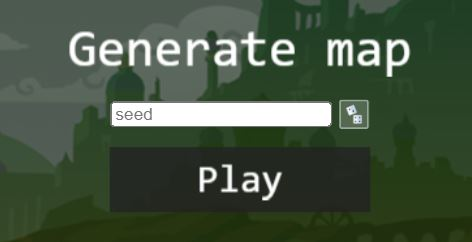
\includegraphics[scale=0.8]{kepek/jatekHasznalat/fomenu}
			\caption{Illusztráció a játék főmenüjéből}
			\label{fig:jatekHasznalat:fomenu}
		\end{figure}
		
		A játék megkezdése után egy másik képernyőn találjuk magunkat, amelyen különféle elemeket láthatunk. Egy példát erre \aref{fig:jatekHasznalat:game_scene} ábrán tekinthetünk meg. Itt különböző tájelemek helyezkednek el, kráterek, fák, és sima fűvel borított területek, ezenkívül pedig egy útvonal. 
		
		\begin{figure}[h!]
			\centering
			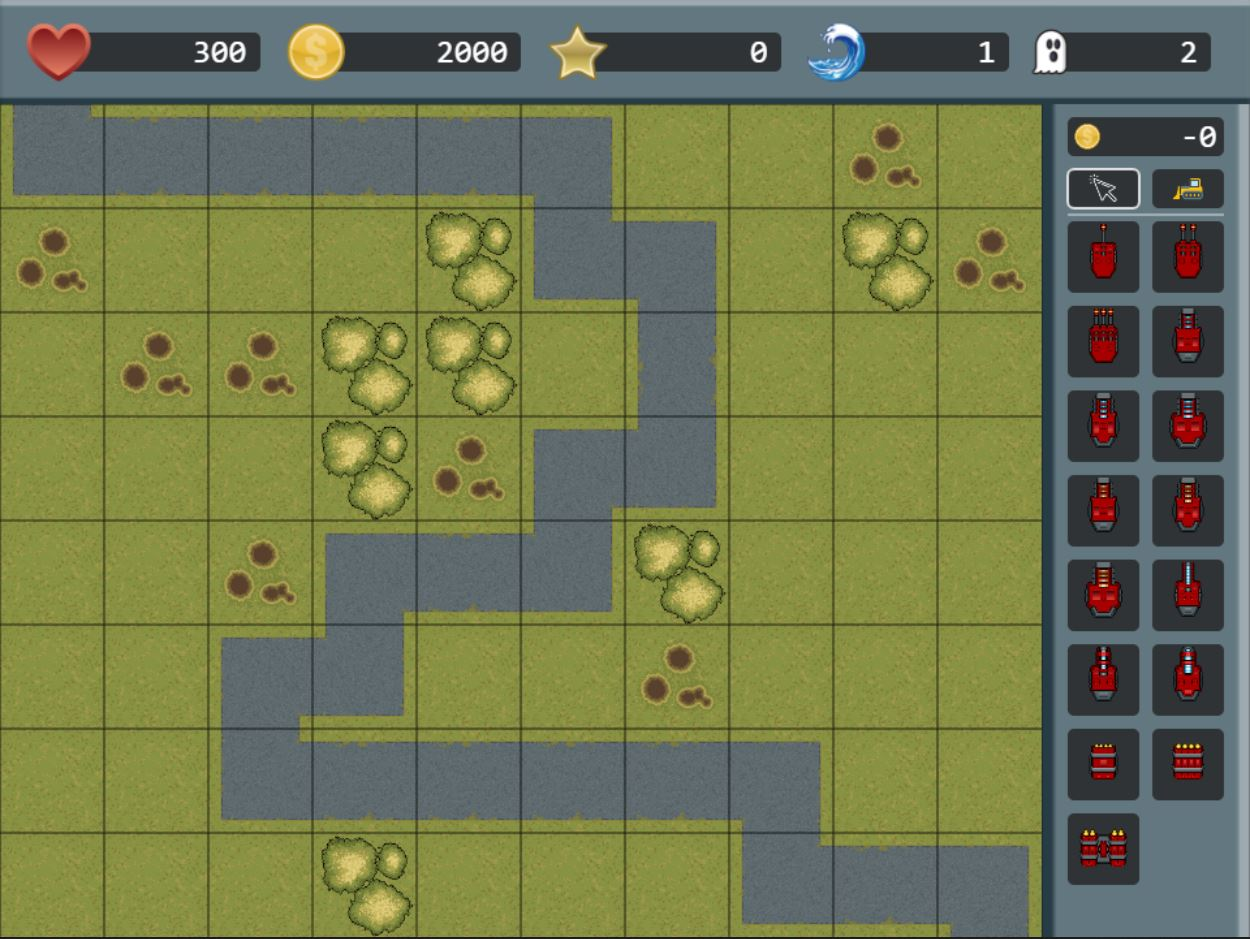
\includegraphics[scale=0.57]{kepek/jatekHasznalat/game_scene}
			\caption{A játék közvetlenül elindítás után}
			\label{fig:jatekHasznalat:game_scene}
		\end{figure}
		
		Az úton szörnyek (lásd: \myref{fig:jatekHasznalat:szorny} ábra) fognak elindulni, pár másodperccel a játék elindítása után, és megpróbálnak végigmenni rajta. A feladatunk az, hogy megakadályozzuk őket ebben. Ezt úgy tudjuk megtenni, hogy különféle tornyokat helyezünk le, ezek fogják sebezni a szörnyeket.
		Az ellenségek feje fölött egy-egy zöld csík látható, amikor megjelennek, ez az életüket szimbolizálja. Amennyiben sebzést szenvednek el, a zöld rész egyre kisebb lesz, amikor pedig teljesen elfogy, a szörny meghal. Az ellenfelek hullámokban, avagy hordaként érkeznek. Minden hullámmal egyre több, és erősebb ellenség fog érkezni.
		
		\begin{figure}[h!]
			\centering
			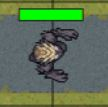
\includegraphics[scale=1.6]{kepek/jatekHasznalat/szorny}
			\caption{A legyőzendő ellenség}
			\label{fig:jatekHasznalat:szorny}
		\end{figure}
		
		Tornyokat csak üres, füves területekre tudunk építeni. Amennyiben nincs már hely ahova tudnánk tenni, le is rombolhatunk előzőleg épülteket, vagy pedig a tájelemeket is. Ezt a jobb oldalt látható felület által tehetjük meg (lásd: \myref{fig:jatekHasznalat:game_scene} ábra jobb oldala).		
		A játék kezdetekor az egér ikont ábrázoló gomb van kijelölve, ekkor ha egy már megépült toronyra rávisszük a kurzort, akkor látni fogunk egy kört körülötte. Ezen a körön belüli távolságra lévő ellenfeleket képes elérni a torony. Ez az egér ikonnal ellátott gomb tehát az úgynevezett "kijelölés mód", ha ezen a módon belül vagyunk, tehát ez a gomb van bekeretezve fehér színnel, akkor egyes objektumokra kattintva a játékon belül nem történik semmi, szimplán amelyik mező felett van a kurzorunk, az lesz kijelölve.
		Az ettől jobbra található, sárga buldózer ábrával ellátott gombra kattintva pedig az "eltávolító mód"-ba kerülünk. Ha ebben a módban vagyunk, és odamozgatjuk a kurzort (kattintás nélkül) egy-egy tárgyra a játékfelületen belül, akkor amíg az adott tárgy fölött van az egerünk, addig az előbb említett gombok feletti rubrikában látható, hogy amennyiben le szeretnénk rombolni az adott objektumot, milyen összeggel változna a pénzünk, avagy aranyunk. Az objektum tényleges eltávolítása kattintásra történik meg.
		Abban az esetben, ha egy korábban megépített tornyot szeretnénk megsemmisíteni, a torony eredeti értékének 60\%-át kapjuk vissza, tehát például ha egy toronyért 1000 aranyat fizettünk, amikor rávisszük a kurzort eltávolító módban, "+600"-at fogunk látni a rubrikában, tehát 600 aranyat kapunk vissza, a rombolás után. Ellenben kráter, vagy fa eltávolításához fizetnünk kell a rombolásért, tehát egy mínusz jel után fog megjelenni az összeg, amennyibe kerül.
		A két gomb alatti felületen különféle tornyok helyezkednek el, 5 különböző típusú toronyot tudunk építeni, és mind az 5 típusból létezik 3 különböző erősségű.
		A tornyok balról jobbra vannak sorbarendezve, tehát adott típusú toronynak először a leggyengébb változát láthatjuk, a végén pedig a legerősebbet, de összességében szituációfüggő is, hogy épp melyik az, amit a legjobban megéri építenünk. Az azonos típusú tornyok hasonló megjelenéssel rendelkeznek, hogy látható legyen az, hogy egy ugyanazon típuson belül helyezkednek el, az áruk azonban különböző.
		
		Az egyes tornyok tulajdonságairól részletes leírás alább, a fejezet végén lévő táblázatokban olvasható.(lásd: \myref{tab:torony_tipus_0}, \myref{tab:torony_tipus_1}, \myref{tab:torony_tipus_2}, \myref{tab:torony_tipus_3}, \myref{tab:torony_tipus_4})
		
		% TODO mindegyik torony - táblázat, a torony képével, képességeivel, árával stb.
		% TODO Tűzgyorsaság (lövés/sec) a lövés / sec az nem igazán hangzik érthetőnek mert több száz az érték és alig lő 2-t  ->2 lövés között 1000/firerate-nyit vár 
		% TODO effekt képességhez - Beletenni a PENETRATION-t  -> átütőképesség
		
	
		A felső felhasználói felületen (lásd \myref{fig:jatekHasznalat:felso_ui} ábra) balról jobbra haladva, a következőket láthatjuk:
		
		\begin{figure}[h!]
			\centering
			
\includegraphics[scale=0.575]{kepek/jatekHasznalat/felso_ui}
			\caption{A felülső felhasználói felület (UI) }
			\label{fig:jatekHasznalat:felso_ui}
		\end{figure}
		
		\begin{itemize}
			\item Piros szív ábra: Az itt látható szám az aktuális életünket jelzi. Ez csökkenni fog, ha egy szörnyet engedünk végigmenni az egész úton. Amikor teljesen elfogy, akkor veszítünk, az adott játék véget ér.
			
			\item Sárga érme "\$" jellel: Ebben a rubrikában az aktuális aranyunk jelenik meg. Ez az érték többször is változhat a játék során. Például toronyépítéskor levonódik a torony összege, ellenben amikor megölünk egy szörnyet akkor kapunk érte adott aranymennyiséget.
			
			\item Csillag ikon: A pillanatnyi összpontszámunkat mutatja. Minden ellenfél megölése után kapunk adott mennyiségű pontot. A végeredményként elért összpontszámot a játék vége után is megtekinthetjuk, mielőtt visszalépünk a főmenübe.
			
			\item Hullám: Azt jelzi, hogy hányadik beérkező hordánál, szörnyhullámnál tartunk éppen.
			
			\item Szellem ikon: A szörnyeket jelképezi. Azt jelzi a játékos számra, hogy az adott hullámban mennyi ellenség érkezik.
		\end{itemize}
	
		A fentieken kívül még megemlítendő, hogy amennyiben olyan tevékenységet kívánunk tenni, amely nem lehetséges az adott mezőben, (például nincs elég pénzünk, hogy megvegyük a jobb oldali menüből kiválasztott tornyot, vagy mondjuk ha az utat próbáljuk meg eltávolítani), úgy a mező pirosas színre vált, ha pedig lehetséges az akció végrehajtása, akkor élénk zöldes árnyalatot kap. (\Aref{fig:jatekHasznalat:kijeloles_minta}. ábrán bal oldalt az előbbi, jobb oldalt pedig az utóbbi látható.)
		
		\begin{figure}[h!]
			\centering
			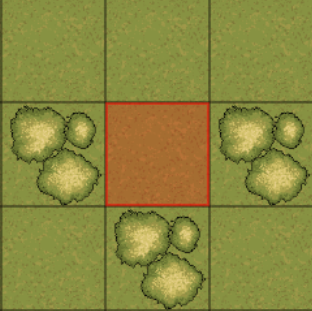
\includegraphics[scale=0.848]{kepek/jatekHasznalat/minta_rossz_kijeloles}
			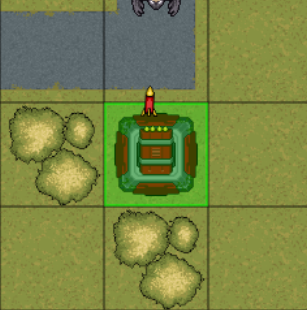
\includegraphics[scale=0.85]{kepek/jatekHasznalat/minta_jo_kijeloles}
			\caption{Minta kijelölésekre - lehetetlen, illetve teljesíthető akciók esetén}
			\label{fig:jatekHasznalat:kijeloles_minta}
		\end{figure}
		
		% game over scene
		
		Most, hogy elolvastuk az előbbieket, már mindent tudunk a játékmenetről. Ami tehát még hátravan, az az, hogy mi történik akkor, amikor esetlegesen elveszítjük az összes életünket, ezáltal a játékot is.
		Ekkor egy új felület jelenik meg előttünk (lásd: \myref{fig:jatekHasznalat:game_over_scene} ábra), amelyen egy "Game Over" felirat taláható, emellett itt megtekinthetjük a játék során elért összpontszámunkat, valamint a "Back to Main Menu" gombra kattintva pedig újra a főmenübe navigálhatjuk magunkat, hogy belekezdhessünk egy új játékmenetbe.
		
		\begin{figure}[h!]
			\centering
			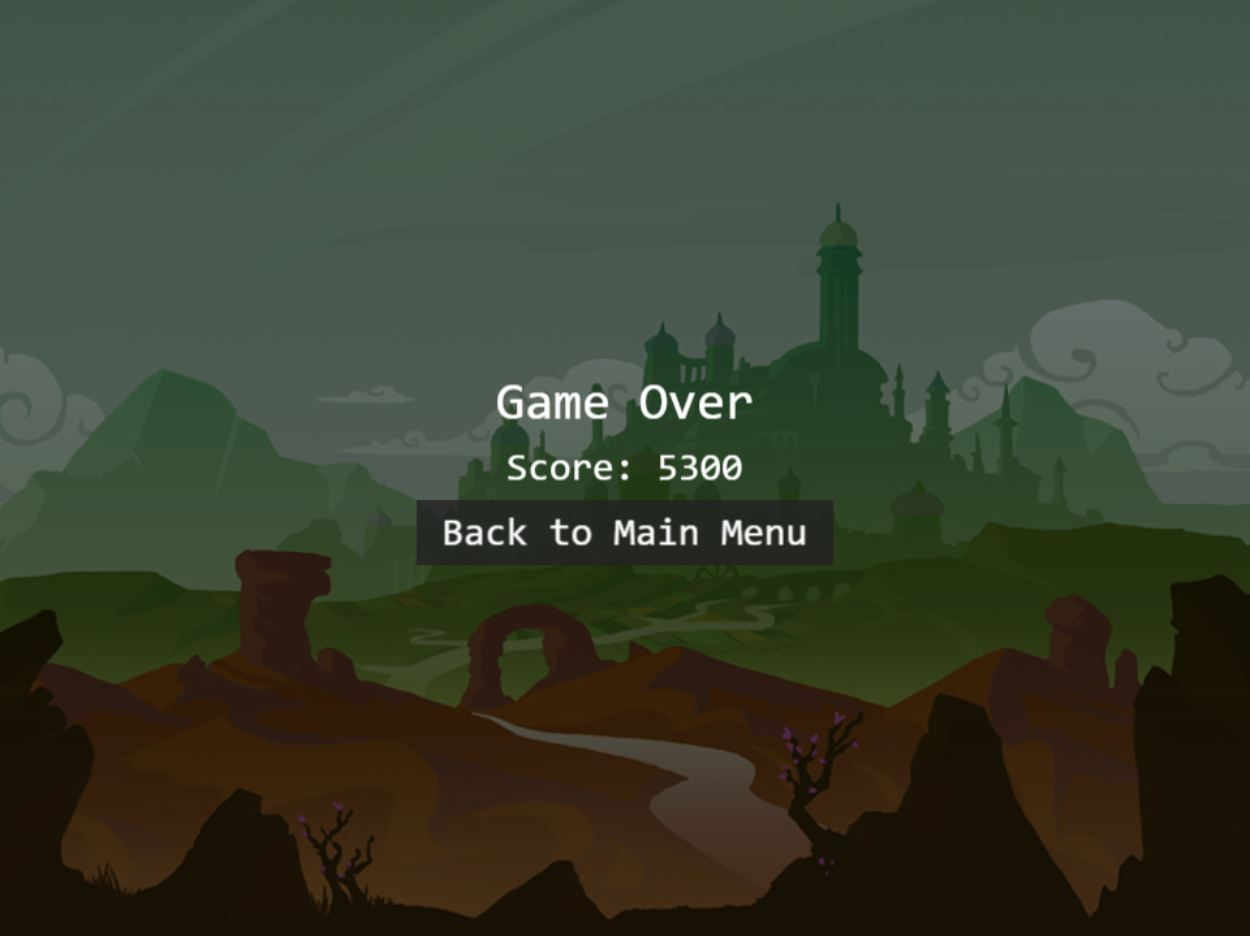
\includegraphics[scale=0.6]{kepek/jatekHasznalat/game_over_scene}
			\caption{Részlet a Game Over képernyőről}
			\label{fig:jatekHasznalat:game_over_scene}
		\end{figure}
	
		\begin{table}[h]
			\centering
			\caption{Első toronytípus tulajdonságai}
			\label{tab:torony_tipus_0}
			\begin{tabular}{|l|c|c|c|}
				\hline
				Kinézet & 
\includegraphics[scale=1.1]{kepek/jatekHasznalat/torony_01} & 
\includegraphics[scale=1.1]{kepek/jatekHasznalat/torony_02} & 
\includegraphics[scale=1.1]{kepek/jatekHasznalat/torony_03} \\ \hline
				Ár (arany) & 500 & 1200 & 3000 \\ \hline
				Maximum lövéstávolság & 220 & 250 & 280 \\ \hline
				Lövés/sec & 2 & 1.6 & 1.4 \\ \hline
				Sebzés & 25 & 25 & 25 \\ \hline
				Százalékos sebzés & Nincs & Nincs & Nincs \\ \hline
				Képesség, effekt & 1 lövedéket lő ki. & \begin{tabular}{@{}c@{}}Egy lövésnél \\ 2 lövedéket lő ki.\end{tabular} & \begin{tabular}{@{}c@{}}Egy lövésnél \\ 3 lövedéket lő ki.\end{tabular} \\ \hline
			\end{tabular}
		\end{table}
		
		\begin{table}[h]
			\centering
			\caption{Második toronytípus tulajdonságai}
			\label{tab:torony_tipus_1}
			\begin{tabular}{|l|c|c|c|}
				\hline
				Kinézet &  &  &  \\ \hline
				Ár (arany) & 800 & 1600 & 3200 \\ \hline
				Maximum lövéstávolság & 220 & 250 & 280 \\ \hline
				Lövés/sec & 1.4 & 1.4 & 1.4 \\ \hline
				Sebzés & 10 & 10 & 10 \\ \hline
				Százalékos sebzés & Nincs & Nincs & Nincs \\ \hline
				Képesség, effekt & \begin{tabular}{@{}c@{}}Lassító \\ lövedéket lő ki.\end{tabular} & \begin{tabular}{@{}c@{}}1-es átütő- \\ képességű lassító \\ lövedéket lő ki.\end{tabular} & \begin{tabular}{@{}c@{}}2-es átütő- \\ képességű lassító \\ lövedéket lő ki.\end{tabular} \\ \hline
			\end{tabular}
		\end{table}
	
		\begin{table}[h]
			\centering
			\caption{Harmadik toronytípus tulajdonságai}
			\label{tab:torony_tipus_2}
			\begin{tabular}{|l|c|c|c|}
				\hline
				Kinézet &  &  &  \\ \hline
				Ár (arany) & 800 & 1600 & 3200 \\ \hline
				Maximum lövéstávolság & 220 & 250 & 280 \\ \hline
				Lövés/sec & 1.4 & 1.4 & 1.4 \\ \hline
				Sebzés & 10 & 10 & 10 \\ \hline
				Százalékos sebzés & Nincs & Nincs & Nincs \\ \hline
				Képesség, effekt & \begin{tabular}{@{}c@{}}Lassító \\ lövedéket lő ki.\end{tabular} & \begin{tabular}{@{}c@{}}1-es átütő- \\ képességű lassító \\ lövedéket lő ki.\end{tabular} & \begin{tabular}{@{}c@{}}2-es átütő- \\ képességű lassító \\ lövedéket lő ki.\end{tabular} \\ \hline
			\end{tabular}
		\end{table}
	
		\begin{table}[h]
			\centering
			\caption{Negyedik toronytípus tulajdonságai}
			\label{tab:torony_tipus_3}
			\begin{tabular}{|l|c|c|c|}
				\hline
				Kinézet &  &  &  \\ \hline
				Ár (arany) & 800 & 1600 & 3200 \\ \hline
				Maximum lövéstávolság & 220 & 250 & 280 \\ \hline
				Lövés/sec & 1.4 & 1.4 & 1.4 \\ \hline
				Sebzés & 10 & 10 & 10 \\ \hline
				Százalékos sebzés & Nincs & Nincs & Nincs \\ \hline
				Képesség, effekt & \begin{tabular}{@{}c@{}}Lassító \\ lövedéket lő ki.\end{tabular} & \begin{tabular}{@{}c@{}}1-es átütő- \\ képességű lassító \\ lövedéket lő ki.\end{tabular} & \begin{tabular}{@{}c@{}}2-es átütő- \\ képességű lassító \\ lövedéket lő ki.\end{tabular} \\ \hline
			\end{tabular}
		\end{table}
	
		\begin{table}[h]
			\centering
			\caption{Ötödik toronytípus tulajdonságai}
			\label{tab:torony_tipus_4}
			\begin{tabular}{|l|c|c|c|}
				\hline
				Kinézet &  &  &  \\ \hline
				Ár (arany) & 800 & 1600 & 3200 \\ \hline
				Maximum lövéstávolság & 220 & 250 & 280 \\ \hline
				Lövés/sec & 1.4 & 1.4 & 1.4 \\ \hline
				Sebzés & 10 & 10 & 10 \\ \hline
				Százalékos sebzés & Nincs & Nincs & Nincs \\ \hline
				Képesség, effekt & \begin{tabular}{@{}c@{}}Lassító \\ lövedéket lő ki.\end{tabular} & \begin{tabular}{@{}c@{}}1-es átütő- \\ képességű lassító \\ lövedéket lő ki.\end{tabular} & \begin{tabular}{@{}c@{}}2-es átütő- \\ képességű lassító \\ lövedéket lő ki.\end{tabular} \\ \hline
			\end{tabular}
		\end{table}
	
	\end{MySection}

\end{MyChapter}
\begin{MyChapter}{Összegzés}
	
	% TODO - elég a legvégén, szerzett tapasztalatok, kihangsúlyozni az elért eredményeket (főleg a sajátokat!), alkalmazás továbbfejlesztési lehetőségei
	
	% TODO Hasonló szerepe van, mint a bevezetésnek. Itt már múltidőben lehet beszélni.	A szerző saját meglátása szerint kell összegezni és értékelni a dolgozat fontosabb eredményeit. Meg lehet benne említeni, hogy mi az ami jobban, mi az ami kevésbé jobban sikerült a tervezettnél. El lehet benne mondani, hogy milyen további tervek, fejlesztési lehetőségek vannak még a témával kapcsolatban.
	
	% TODO összegzésben Phaser 3-mal kapcsolatos tapasztalatokat(általánosan h erre a célra mennyire felel meg, ajánlanám-e ezt ilyen jellegű program készítésére)
	
	% TODO Továbbfejlesztése lehetoseg:	Ui-ra információs dialóg amikor a torony stb felé visszük az egeret
	
	% TODO ### Továbbfejlesztés ###
	% - hangok kimaradtak
	% - teljes tesztlefedettsége, pl az objectekre is
	% - a konfigurálthaót értékeket egy külső fájlból betölteni így manuálisan akár a felhasználó is módosíthatja az értékeket saját kénye kedve szerint.
	% - effektekhez vizuális részt is adni, pl a slow esetén megfagyvottként látszódjon a enemy.
	
	% TODO továbbfejlesztés:
	% - Finomhangolási értékeken lehetne még módosítani, mert tapasztalat alapján elég könnyűre sikerült, de ez akár egy különálló kutatás tárgyát is képezhetné, hiszen a tökéletes egyensúly megtalálsa egy optimalizálási feladatként is felfogható.
	% - Ha több féle, különböző képességű enemy lenne, akkor nehezebb lenne / újra kellene finomhangolni.
\end{MyChapter}

% !TEX encoding = UTF-8 Unicode

\begin{thebibliography}{x}
	\addcontentsline{toc}{chapter}{\bibname}

	
	\bibitem{Video_game_development}
	{https://en.wikipedia.org/wiki/Video\_game\_development} \\
	Wikipedia, the free encyclopedia

% TODO add bibliography items
% EXAMPLE:
% % https://users.iit.uni-miskolc.hu/~mileff/grafika/Grafika_programozasa_jegyzet_v0.66_Mileff_P.pdf
% \bibitem{mileff}
% Mileff Péter: \emph{Grafika programozása}, tárgyi jegyzet, \\
% Miskolci Egyetem, Általános Informatikai Tanszék, 2015.

\end{thebibliography}


% !TEX encoding = UTF-8 Unicode
\newpage

\section*{CD-melléklet tartalma}
% használati útmutató megír

A szakdolgozat \LaTeX\ segítségével készült. A dolgozat forrásfájljai a \texttt{report/sources} mappában találhatóak.
A dolgozat PDF-re fordított változata pedig a \texttt{report/pdf} mappában található meg \texttt{report.pdf} néven.

A dolgozat során elkészült játék forrásfájljai a \texttt{game/sources} mappába kerültek elhelyezésre.
A program fordításához a \textit{Node.js}-re, \textit{NPM csomagkezelő}-re, illetve internetkapcsolatra van szükség.

A \texttt{game/sources} mappában egy konzolt szükséges először nyitni, itt az \texttt{npm install} parancsot kell futtatni, a szükséges függőségek telepítéséhez (ehhez internetkapcsolat szükséges).
Ezután ha a teszteket szeretnénk futtatni, akkor azt az \texttt{npm test} parancs segítségével tehetjük meg.
Az alkalmazás fejlesztői módban való elindításához az \texttt{npm start} parancsot kell futtatnunk, ami a fordítás után egy webszervert fog elindítani a gépünkön a $8080$-as porton. Ezután böngészőnkben a \url{localhost:8080} -as oldalra navigálva elérhetjük az alkalmazást.
A program optimalizáltan és kiadható formában fordított változatát az \texttt{npm run build} parancs futtatásával lehet elkészíteni. Ez az aktuális mappán belüli \texttt{dist} mappába fogja elhelyezni a fordított fájlokat. Ezt követően a kész fájlokat egy webszerverre másolva lehet használni. A kipróbálhatóság érdekében az \texttt{npm run serve-build} paranccsal tudunk futtatni ideiglenesen egy minimális funkciókkal bíró webszervert. Ez a parancs elméletileg az alapértelmezett böngészőnkben meg is nyitja az alkalmazást mely a \url{http://127.0.0.1:4949/dist/} címen érhető el.

Az előre lefordított alkalmazás a \texttt{game/dist} mappában található, ennek használatához előzőekben említetthez hasonlóan szükségünk van egy webszerverre.

A játék használatáról részletesebben a dolgozatban a \myref{Használat} fejezetben található útmutatás.


\end{document}
